% Options for packages loaded elsewhere
% Options for packages loaded elsewhere
\PassOptionsToPackage{unicode}{hyperref}
\PassOptionsToPackage{hyphens}{url}
\PassOptionsToPackage{dvipsnames,svgnames,x11names}{xcolor}
%
\documentclass[
  a4paper,
  DIV=11,
  numbers=noendperiod]{scrreprt}
\usepackage{xcolor}
\usepackage[margin=1in]{geometry}
\usepackage{amsmath,amssymb}
\setcounter{secnumdepth}{5}
\usepackage{iftex}
\ifPDFTeX
  \usepackage[T1]{fontenc}
  \usepackage[utf8]{inputenc}
  \usepackage{textcomp} % provide euro and other symbols
\else % if luatex or xetex
  \usepackage{unicode-math} % this also loads fontspec
  \defaultfontfeatures{Scale=MatchLowercase}
  \defaultfontfeatures[\rmfamily]{Ligatures=TeX,Scale=1}
\fi
\usepackage{lmodern}
\ifPDFTeX\else
  % xetex/luatex font selection
\fi
% Use upquote if available, for straight quotes in verbatim environments
\IfFileExists{upquote.sty}{\usepackage{upquote}}{}
\IfFileExists{microtype.sty}{% use microtype if available
  \usepackage[]{microtype}
  \UseMicrotypeSet[protrusion]{basicmath} % disable protrusion for tt fonts
}{}
\makeatletter
\@ifundefined{KOMAClassName}{% if non-KOMA class
  \IfFileExists{parskip.sty}{%
    \usepackage{parskip}
  }{% else
    \setlength{\parindent}{0pt}
    \setlength{\parskip}{6pt plus 2pt minus 1pt}}
}{% if KOMA class
  \KOMAoptions{parskip=half}}
\makeatother
% Make \paragraph and \subparagraph free-standing
\makeatletter
\ifx\paragraph\undefined\else
  \let\oldparagraph\paragraph
  \renewcommand{\paragraph}{
    \@ifstar
      \xxxParagraphStar
      \xxxParagraphNoStar
  }
  \newcommand{\xxxParagraphStar}[1]{\oldparagraph*{#1}\mbox{}}
  \newcommand{\xxxParagraphNoStar}[1]{\oldparagraph{#1}\mbox{}}
\fi
\ifx\subparagraph\undefined\else
  \let\oldsubparagraph\subparagraph
  \renewcommand{\subparagraph}{
    \@ifstar
      \xxxSubParagraphStar
      \xxxSubParagraphNoStar
  }
  \newcommand{\xxxSubParagraphStar}[1]{\oldsubparagraph*{#1}\mbox{}}
  \newcommand{\xxxSubParagraphNoStar}[1]{\oldsubparagraph{#1}\mbox{}}
\fi
\makeatother

\usepackage{color}
\usepackage{fancyvrb}
\newcommand{\VerbBar}{|}
\newcommand{\VERB}{\Verb[commandchars=\\\{\}]}
\DefineVerbatimEnvironment{Highlighting}{Verbatim}{commandchars=\\\{\}}
% Add ',fontsize=\small' for more characters per line
\usepackage{framed}
\definecolor{shadecolor}{RGB}{241,243,245}
\newenvironment{Shaded}{\begin{snugshade}}{\end{snugshade}}
\newcommand{\AlertTok}[1]{\textcolor[rgb]{0.68,0.00,0.00}{#1}}
\newcommand{\AnnotationTok}[1]{\textcolor[rgb]{0.37,0.37,0.37}{#1}}
\newcommand{\AttributeTok}[1]{\textcolor[rgb]{0.40,0.45,0.13}{#1}}
\newcommand{\BaseNTok}[1]{\textcolor[rgb]{0.68,0.00,0.00}{#1}}
\newcommand{\BuiltInTok}[1]{\textcolor[rgb]{0.00,0.23,0.31}{#1}}
\newcommand{\CharTok}[1]{\textcolor[rgb]{0.13,0.47,0.30}{#1}}
\newcommand{\CommentTok}[1]{\textcolor[rgb]{0.37,0.37,0.37}{#1}}
\newcommand{\CommentVarTok}[1]{\textcolor[rgb]{0.37,0.37,0.37}{\textit{#1}}}
\newcommand{\ConstantTok}[1]{\textcolor[rgb]{0.56,0.35,0.01}{#1}}
\newcommand{\ControlFlowTok}[1]{\textcolor[rgb]{0.00,0.23,0.31}{\textbf{#1}}}
\newcommand{\DataTypeTok}[1]{\textcolor[rgb]{0.68,0.00,0.00}{#1}}
\newcommand{\DecValTok}[1]{\textcolor[rgb]{0.68,0.00,0.00}{#1}}
\newcommand{\DocumentationTok}[1]{\textcolor[rgb]{0.37,0.37,0.37}{\textit{#1}}}
\newcommand{\ErrorTok}[1]{\textcolor[rgb]{0.68,0.00,0.00}{#1}}
\newcommand{\ExtensionTok}[1]{\textcolor[rgb]{0.00,0.23,0.31}{#1}}
\newcommand{\FloatTok}[1]{\textcolor[rgb]{0.68,0.00,0.00}{#1}}
\newcommand{\FunctionTok}[1]{\textcolor[rgb]{0.28,0.35,0.67}{#1}}
\newcommand{\ImportTok}[1]{\textcolor[rgb]{0.00,0.46,0.62}{#1}}
\newcommand{\InformationTok}[1]{\textcolor[rgb]{0.37,0.37,0.37}{#1}}
\newcommand{\KeywordTok}[1]{\textcolor[rgb]{0.00,0.23,0.31}{\textbf{#1}}}
\newcommand{\NormalTok}[1]{\textcolor[rgb]{0.00,0.23,0.31}{#1}}
\newcommand{\OperatorTok}[1]{\textcolor[rgb]{0.37,0.37,0.37}{#1}}
\newcommand{\OtherTok}[1]{\textcolor[rgb]{0.00,0.23,0.31}{#1}}
\newcommand{\PreprocessorTok}[1]{\textcolor[rgb]{0.68,0.00,0.00}{#1}}
\newcommand{\RegionMarkerTok}[1]{\textcolor[rgb]{0.00,0.23,0.31}{#1}}
\newcommand{\SpecialCharTok}[1]{\textcolor[rgb]{0.37,0.37,0.37}{#1}}
\newcommand{\SpecialStringTok}[1]{\textcolor[rgb]{0.13,0.47,0.30}{#1}}
\newcommand{\StringTok}[1]{\textcolor[rgb]{0.13,0.47,0.30}{#1}}
\newcommand{\VariableTok}[1]{\textcolor[rgb]{0.07,0.07,0.07}{#1}}
\newcommand{\VerbatimStringTok}[1]{\textcolor[rgb]{0.13,0.47,0.30}{#1}}
\newcommand{\WarningTok}[1]{\textcolor[rgb]{0.37,0.37,0.37}{\textit{#1}}}

\usepackage{longtable,booktabs,array}
\usepackage{calc} % for calculating minipage widths
% Correct order of tables after \paragraph or \subparagraph
\usepackage{etoolbox}
\makeatletter
\patchcmd\longtable{\par}{\if@noskipsec\mbox{}\fi\par}{}{}
\makeatother
% Allow footnotes in longtable head/foot
\IfFileExists{footnotehyper.sty}{\usepackage{footnotehyper}}{\usepackage{footnote}}
\makesavenoteenv{longtable}
\usepackage{graphicx}
\makeatletter
\newsavebox\pandoc@box
\newcommand*\pandocbounded[1]{% scales image to fit in text height/width
  \sbox\pandoc@box{#1}%
  \Gscale@div\@tempa{\textheight}{\dimexpr\ht\pandoc@box+\dp\pandoc@box\relax}%
  \Gscale@div\@tempb{\linewidth}{\wd\pandoc@box}%
  \ifdim\@tempb\p@<\@tempa\p@\let\@tempa\@tempb\fi% select the smaller of both
  \ifdim\@tempa\p@<\p@\scalebox{\@tempa}{\usebox\pandoc@box}%
  \else\usebox{\pandoc@box}%
  \fi%
}
% Set default figure placement to htbp
\def\fps@figure{htbp}
\makeatother


% definitions for citeproc citations
\NewDocumentCommand\citeproctext{}{}
\NewDocumentCommand\citeproc{mm}{%
  \begingroup\def\citeproctext{#2}\cite{#1}\endgroup}
\makeatletter
 % allow citations to break across lines
 \let\@cite@ofmt\@firstofone
 % avoid brackets around text for \cite:
 \def\@biblabel#1{}
 \def\@cite#1#2{{#1\if@tempswa , #2\fi}}
\makeatother
\newlength{\cslhangindent}
\setlength{\cslhangindent}{1.5em}
\newlength{\csllabelwidth}
\setlength{\csllabelwidth}{3em}
\newenvironment{CSLReferences}[2] % #1 hanging-indent, #2 entry-spacing
 {\begin{list}{}{%
  \setlength{\itemindent}{0pt}
  \setlength{\leftmargin}{0pt}
  \setlength{\parsep}{0pt}
  % turn on hanging indent if param 1 is 1
  \ifodd #1
   \setlength{\leftmargin}{\cslhangindent}
   \setlength{\itemindent}{-1\cslhangindent}
  \fi
  % set entry spacing
  \setlength{\itemsep}{#2\baselineskip}}}
 {\end{list}}
\usepackage{calc}
\newcommand{\CSLBlock}[1]{\hfill\break\parbox[t]{\linewidth}{\strut\ignorespaces#1\strut}}
\newcommand{\CSLLeftMargin}[1]{\parbox[t]{\csllabelwidth}{\strut#1\strut}}
\newcommand{\CSLRightInline}[1]{\parbox[t]{\linewidth - \csllabelwidth}{\strut#1\strut}}
\newcommand{\CSLIndent}[1]{\hspace{\cslhangindent}#1}



\setlength{\emergencystretch}{3em} % prevent overfull lines

\providecommand{\tightlist}{%
  \setlength{\itemsep}{0pt}\setlength{\parskip}{0pt}}



 


\KOMAoption{captions}{tableheading}
\makeatletter
\@ifpackageloaded{bookmark}{}{\usepackage{bookmark}}
\makeatother
\makeatletter
\@ifpackageloaded{caption}{}{\usepackage{caption}}
\AtBeginDocument{%
\ifdefined\contentsname
  \renewcommand*\contentsname{Table of contents}
\else
  \newcommand\contentsname{Table of contents}
\fi
\ifdefined\listfigurename
  \renewcommand*\listfigurename{List of Figures}
\else
  \newcommand\listfigurename{List of Figures}
\fi
\ifdefined\listtablename
  \renewcommand*\listtablename{List of Tables}
\else
  \newcommand\listtablename{List of Tables}
\fi
\ifdefined\figurename
  \renewcommand*\figurename{Figure}
\else
  \newcommand\figurename{Figure}
\fi
\ifdefined\tablename
  \renewcommand*\tablename{Table}
\else
  \newcommand\tablename{Table}
\fi
}
\@ifpackageloaded{float}{}{\usepackage{float}}
\floatstyle{ruled}
\@ifundefined{c@chapter}{\newfloat{codelisting}{h}{lop}}{\newfloat{codelisting}{h}{lop}[chapter]}
\floatname{codelisting}{Listing}
\newcommand*\listoflistings{\listof{codelisting}{List of Listings}}
\makeatother
\makeatletter
\makeatother
\makeatletter
\@ifpackageloaded{caption}{}{\usepackage{caption}}
\@ifpackageloaded{subcaption}{}{\usepackage{subcaption}}
\makeatother
\usepackage{bookmark}
\IfFileExists{xurl.sty}{\usepackage{xurl}}{} % add URL line breaks if available
\urlstyle{same}
\hypersetup{
  pdftitle={Interval Forecasting of Cryptocurrency Returns using Quantile Regression Forests: An Application to the Solana Ecosystem},
  pdfauthor={James Lewis},
  colorlinks=true,
  linkcolor={blue},
  filecolor={Maroon},
  citecolor={Blue},
  urlcolor={Blue},
  pdfcreator={LaTeX via pandoc}}


\title{Interval Forecasting of Cryptocurrency Returns using Quantile
Regression Forests: An Application to the Solana Ecosystem}
\usepackage{etoolbox}
\makeatletter
\providecommand{\subtitle}[1]{% add subtitle to \maketitle
  \apptocmd{\@title}{\par {\large #1 \par}}{}{}
}
\makeatother
\subtitle{Interval Forecasting of Cryptocurrency Returns using Quantile
Regression Forests: An Application to the Solana Ecosystem}
\author{James Lewis}
\date{}
\begin{document}
\maketitle

\renewcommand*\contentsname{Table of contents}
{
\hypersetup{linkcolor=}
\setcounter{tocdepth}{2}
\tableofcontents
}

\bookmarksetup{startatroot}

\chapter{Abstract}\label{abstract}

Interval Forecasting of Cryptocurrency Returns using Quantile Regression
Forests: An Application to the Solana Ecosystem

\hfill\break

\textbf{Abstract.} (200--300 words placeholder) Problem, data (12-h
bars; 72-h target), models (QRF, LQR, LGBM), rolling CV (120/24/6),
metrics (pinball, coverage, width), key results + trading relevance.

\bookmarksetup{startatroot}

\chapter{Introduction}\label{introduction}

\subsection{The Economic Challenge of Forecasting in Emerging
Ecosystems}\label{the-economic-challenge-of-forecasting-in-emerging-ecosystems}

Extreme volatility and non-normal return distributions are defining
characteristics of cryptocurrency markets, rendering traditional point
forecasts insufficient for robust risk management
(\citeproc{ref-Gkillas2018}{Gkillas and Katsiampa, 2018}). This
challenge is particularly acute for mid-capitalisation tokens within
emerging ecosystems like Solana. Unlike large-cap assets, these tokens
are subject to rapid narrative shifts and idiosyncratic on-chain
dynamics; yet unlike micro-caps, they are liquid enough to attract
significant capital. For participants in this space, standard risk
models often fail during periods of high network activity or
ecosystem-wide events, creating a clear demand for forecasting tools
that can dynamically price tail risk.

This dissertation argues that the primary objective must shift from
point prediction to \textbf{interval forecasting}. By generating
calibrated prediction intervals through conditional quantiles, we can
capture the asymmetry and tail risk inherent in these volatile assets. A
well-calibrated lower quantile serves as a dynamic, forward-looking
analogue to Value-at-Risk (VaR) (\citeproc{ref-Engle2004}{Engle and
Manganelli, 2004}), while the upper quantile informs on potential
upside, providing a comprehensive basis for sophisticated risk
management and tactical decision-making.

\subsection{A Principled Approach: Quantile
Regression}\label{a-principled-approach-quantile-regression}

To construct reliable prediction intervals, we adopt the framework of
\textbf{quantile regression} (\citeproc{ref-Koenker1978}{Koenker and
Bassett, 1978}). This approach is formally grounded in the
\textbf{pinball loss function}, a proper scoring rule that is uniquely
minimised when the forecast matches the true conditional quantile of the
distribution. For a target outcome \(y\) and a forecast for the
\(\tau\)-th quantile, \(\hat{q}_{\tau}\), the loss is:

\[L_{\tau}(y, \hat{q}_{\tau}) = (\tau - \mathbf{1}\{y < \hat{q}_{\tau}\})(y - \hat{q}_{\tau})\]

This allows models to be evaluated on two critical properties:
\textbf{calibration} (does an 80\% interval contain the outcome 80\% of
the time?) and \textbf{sharpness} (are the intervals as narrow as
possible while maintaining calibration?)
(\citeproc{ref-Gneiting2007}{Gneiting and Raftery, 2007}). These
properties are paramount in crypto markets, where accurately quantifying
both risk and opportunity is the basis of effective strategy.

\subsection{The State of the Art and the Research
Gap}\label{the-state-of-the-art-and-the-research-gap}

The literature on cryptocurrency forecasting has largely bifurcated. One
branch applies econometric models like GARCH, which excel at modelling
volatility but are constrained by parametric assumptions
(\citeproc{ref-Bollerslev1986}{Bollerslev, 1986}). The other employs
machine learning, but predominantly for point forecasting of price or
direction (\citeproc{ref-Mcnally2018}{Mcnally, Roche and Caton, 2018}).
While some studies have applied quantile regression to major
crypto-assets (\citeproc{ref-Catania2019}{Catania and Sandholdt, 2019}),
they have typically relied on simpler linear models or have not fully
leveraged the rich feature set available from on-chain data.
Furthermore, the critical step of post-hoc calibration to ensure nominal
coverage guarantees, especially for non-parametric methods, is often
overlooked.

This dissertation is designed to address these gaps by making three core
contributions: it shifts the focus from point prediction to
distributional accuracy; it applies a sophisticated non-parametric
methodology to the under-researched domain of mid-cap altcoins; and it
integrates a rich, multi-domain feature set that explicitly includes
on-chain activity.

\subsection{1.4 Problem Formulation: The Solana
Ecosystem}\label{problem-formulation-the-solana-ecosystem}

This study focuses on forecasting \textbf{72-hour log-returns} for a
universe of mid-cap tokens within the Solana ecosystem, using data
aggregated in 12-hour intervals. The asset universe comprises tokens
with a market capitalisation exceeding \textbackslash\$30 million,
ensuring a focus on liquid yet idiosyncratic assets. The forecasting
model is built upon a feature set designed to capture the multi-faceted
drivers of returns, spanning five domains: (i) \textbf{momentum}, (ii)
\textbf{volatility}, (iii) \textbf{market microstructure}, (iv)
\textbf{on-chain activity}, and (v) \textbf{cross-asset context}.

\subsection{Methodology and
Contributions}\label{methodology-and-contributions}

The central hypothesis is that the non-linear, interaction-heavy nature
of this market demands a non-parametric approach. We propose an adapted
\textbf{Quantile Regression Forests (QRF)} model
(\citeproc{ref-Meinshausen2006}{Meinshausen, 2006}). QRF was selected as
the primary model for several reasons. Firstly, its ensemble nature
provides inherent robustness to the noisy predictors common in
high-dimensional financial feature sets. Secondly, unlike gradient
boosting, QRF's independent tree construction can be less prone to
overfitting in non-stationary environments. Finally, its method of
estimating quantiles from the full distribution of training samples in
terminal nodes is a more direct and empirically stable approach than
methods requiring separate models for each quantile. To tailor the model
for financial time series, we incorporate several critical enhancements:
\textbf{time-decay weighting} to prioritise recent data,
\textbf{volatility regime offsets} to adapt to changing market
conditions, and \textbf{isotonic regression} to enforce the theoretical
non-crossing of quantiles.

We benchmark our adapted QRF against a parametric \textbf{Linear
Quantile Regression (LQR)} and a powerful \textbf{LightGBM} model
(\citeproc{ref-Ke2017}{Ke \emph{et al.}, 2017}) augmented with
\textbf{conformal prediction} (\citeproc{ref-Romano2019}{Romano,
Patterson and Candès, 2019}). Preliminary results suggest that the
primary advantage of the adapted QRF framework lies in its superior
ability to synthesise on-chain activity and market microstructure
features to anticipate shifts in return distribution skewness---a
dynamic that linear models fail to capture.

\subsection{Scope and Delimitations}\label{scope-and-delimitations}

This dissertation provides a rigorous methodological and empirical
analysis of interval forecasting. It does not aim to develop a complete,
production-ready trading system, which would require further
considerations such as transaction costs, liquidity constraints, and
execution latency. Furthermore, the feature set, while comprehensive, is
confined to publicly available market and on-chain data, thereby
excluding alternative data sources such as social media sentiment or
developer activity metrics, which may also contain predictive
information. The findings are specific to the mid-cap tokens within the
Solana ecosystem during the observation period and may not be directly
generalisable to other blockchains, market-cap tiers, or market regimes
without further investigation and potential recalibration.

\subsection{Research Question}\label{research-question}

This framework motivates the central research question of this
dissertation:

\textbf{Can an adapted Quantile Regression Forest model deliver sharper
and better-calibrated prediction intervals for 72-hour returns of
mid-cap Solana tokens compared to standard linear and gradient-boosted
quantile regression baselines?}

This overarching question is decomposed into four specific, testable
hypotheses:

\begin{enumerate}
\def\labelenumi{\arabic{enumi}.}
\item
  Superior Accuracy: The proposed QRF model achieves a lower mean
  pinball loss across the quantile spectrum than both LQR and LightGBM
  with conformal prediction.
\item
  Superior Calibration: The QRF model's empirical coverage rates for
  80\% and 90\% intervals are closer to their nominal levels.
\item
  Superior Sharpness: The QRF model produces narrower prediction
  intervals than the conformally-adjusted LightGBM model, without
  sacrificing calibration.
\item
  Statistical Significance: The performance improvements offered by QRF
  are statistically significant as determined by formal tests on pinball
  loss differentials.
\end{enumerate}

\subsection{Dissertation Outline}\label{dissertation-outline}

The remainder of this dissertation unfolds as follows. Chapter 2
establishes the theoretical context by reviewing the relevant
literature. Chapter 3 details the data pipeline and feature engineering
process, while Chapter 4 outlines the core methodology. The empirical
analysis begins in Chapter 5 with the main comparative results, which
are translated into a practical trading application in Chapter 6 and
stress-tested for robustness in Chapter 7. Finally, Chapter 8 discusses
the broader implications, leading to the conclusion in Chapter 9, which
summarises the contributions and suggests avenues for future research.

\bookmarksetup{startatroot}

\chapter{Literature Review}\label{literature-review}

This chapter provides a critical review of the literature that justifies
the methodology of this dissertation. It first establishes the unique
statistical properties of cryptocurrency returns that necessitate
specialised forecasting approaches. The review then evaluates the
relative merits of parametric and non-parametric quantile estimation
models, before examining the essential frameworks for robust forecast
evaluation, calibration, and comparison. The chapter synthesises these
distinct strands of literature to build a coherent argument for the
selection of an adapted Quantile Regression Forest as the core model,
and for the specific methodological refinements required for its
application.

\subsection{The Challenge: Statistical Properties of Cryptocurrency
Returns}\label{the-challenge-statistical-properties-of-cryptocurrency-returns}

The return distributions of cryptocurrencies are characterised by heavy
tails, significant skew, and extreme kurtosis relative to traditional
assets, reflecting the frequency of large, abrupt price movements
(\citeproc{ref-Gkillas2018}{Gkillas and Katsiampa, 2018}). This
leptokurtosis is compounded by pronounced volatility
clustering---periods of relative calm followed by explosive
variability---a dynamic exacerbated by the market's continuous operation
and fragmented liquidity, which can amplify shocks across uncoordinated
venues.

Crucially, this extreme risk is also largely idiosyncratic to the crypto
market. Major cryptocurrencies carry substantial tail risk that is not
strongly correlated with traditional stock market indices; instead,
extreme events are driven by crypto-specific factors such as investor
sentiment, regulatory news, or network-level events
(\citeproc{ref-Borri2019}{Borri, 2019}). Furthermore, their returns show
little to no exposure to standard macroeconomic risk factors, being
influenced instead by internal drivers like network momentum and
adoption metrics (\citeproc{ref-Liu2021}{Liu and Tsyvinski, 2021}). This
body of evidence demonstrates that classical financial risk models, with
their reliance on Gaussian assumptions and traditional risk factors, are
fundamentally misspecified for crypto assets. A credible forecasting
framework must therefore abandon these assumptions and be built to
incorporate the crypto-native features that drive risk.

\subsection{Approaches to Quantile
Estimation}\label{approaches-to-quantile-estimation}

Given the non-normal character of crypto returns established previously,
estimating the full conditional distribution is more informative than
forecasting its central tendency. Quantile regression provides a natural
framework for this, but the choice between a restrictive parametric
model and a flexible non-parametric one is critical.

\subsubsection{The Parametric Benchmark: Linear Quantile
Regression}\label{the-parametric-benchmark-linear-quantile-regression}

Quantile regression, introduced by (\citeproc{ref-Koenker1978}{Koenker
and Bassett, 1978}), generalises linear regression by estimating
conditional quantiles directly. For a given quantile level
\(\tau \in (0,1)\), the linear quantile regression (LQR) estimator
solves:

\[\hat{\beta}_\tau = \arg\min_{\beta} \sum_{i=1}^{n} \rho_\tau(y_i - x_i^\top\beta)\]

where \(\rho_\tau(u) = u(\tau - \mathbb{1}\{u<0\})\) is the
\textbf{pinball loss function}. While LQR provides a transparent and
interpretable benchmark, its fundamental assumption of a fixed linear
relationship across all quantiles represents a severe limitation. This
rigidity is fundamentally at odds with the non-linear volatility
dynamics and abrupt regime shifts that define cryptocurrency markets.
Furthermore, the common practical issue of \textbf{quantile
crossing}---where independently estimated quantile lines intersect---can
yield incoherent and unusable interval forecasts unless post-hoc
remedies like rearrangement are applied
(\citeproc{ref-Chernozhukov2010}{Chernozhukov, Fernández-Val and
Galichon, 2010}). These shortcomings do not merely motivate, but
necessitate the exploration of more flexible, non-parametric methods.

\subsubsection{Non-Parametric Solutions: Quantile Regression
Forests}\label{non-parametric-solutions-quantile-regression-forests}

As a direct response to the limitations of linear models, Quantile
Regression Forests (QRF), proposed by
(\citeproc{ref-Meinshausen2006}{Meinshausen, 2006}), extend the Random
Forest algorithm (\citeproc{ref-Breiman2001}{Breiman, 2001}) to estimate
the entire conditional distribution. Instead of averaging outcomes in
terminal nodes, QRF uses the full empirical distribution of training
responses within the leaves to form a predictive distribution, from
which conditional quantiles are derived.

This non-parametric approach is inherently well-suited to financial
data; it naturally captures complex non-linearities and adapts to
heteroskedasticity without pre-specification. However, QRF is not
without its own challenges. Its theoretical foundation rests on an
assumption of independent and identically distributed (i.i.d.) data---a
condition clearly violated by financial time series. A naive application
of QRF to time-ordered data can therefore lead to biased estimates. This
violation is a central methodological challenge that requires specific
adaptations, such as the time-decay weighting and rolling validation
schemes discussed later, to apply the model soundly. Furthermore, the
accuracy of its tail quantile estimates can degrade if the terminal
leaves are sparsely populated, a genuine risk when modelling extreme
events. Boosting offers another route to non-parametric quantile
estimation, but with contrasting properties.

\subsubsection{A Boosting Alternative: LightGBM for
Quantiles}\label{a-boosting-alternative-lightgbm-for-quantiles}

Gradient boosting presents another powerful non-parametric paradigm. It
constructs an ensemble sequentially, with each new tree trained to
correct the errors---specifically, the gradients of the loss
function---of the preceding models
(\citeproc{ref-Friedman2001}{Friedman, 2001}). This methodology can be
directly applied to quantile regression by using the pinball loss as the
objective. LightGBM (\citeproc{ref-Ke2017}{Ke \emph{et al.}, 2017}) is a
highly efficient and scalable implementation of this idea, making it a
formidable baseline.

In sharp contrast to QRF's parallelised construction, boosting's
sequential focus on difficult-to-predict instances can yield sharper
estimates in the tails. This potential for higher accuracy, however,
comes with significant trade-offs. A separate model must typically be
trained for each target quantile, imposing a considerable computational
burden. The aggressive, error-focused fitting can also produce
``ragged'' and unstable quantile estimates in regions with sparse data
and may overfit transient noise without careful regularisation. Finally,
like LQR, independently fitted boosting models are susceptible to the
problem of quantile crossing.

\subsection{Ensuring Rigour: Calibration, Evaluation, and
Comparison}\label{ensuring-rigour-calibration-evaluation-and-comparison}

Selecting a flexible forecasting model is insufficient on its own; its
predictive performance must be evaluated using principled metrics, its
outputs calibrated to ensure reliability, and its superiority over
alternatives established through formal statistical tests.

\subsubsection{Proper Scoring and Forecast
Evaluation}\label{proper-scoring-and-forecast-evaluation}

A principled evaluation of probabilistic forecasts requires the use of
\textbf{strictly proper scoring rules}, which incentivise the model to
report its true belief about the future distribution. For quantile
forecasts, the canonical proper scoring rule is the pinball loss
(\citeproc{ref-Gneiting2007}{Gneiting and Raftery, 2007}). As the metric
being directly optimised by the models, it serves as the primary tool
for evaluation. However, performance is not a single dimension. The
quality of an interval forecast is judged by two distinct and often
competing properties: \textbf{calibration}, the statistical consistency
between the nominal coverage rate (e.g., 90\%) and the empirical
frequency of outcomes falling within the interval; and
\textbf{sharpness}, the narrowness of the interval. An ideal forecast is
one that is maximally sharp, subject to being well-calibrated. However,
a model optimised on a proper score is not inherently guaranteed to be
well-calibrated in finite samples. This gap between theoretical
optimisation and empirical reliability motivates the use of formal
calibration techniques.

\subsubsection{Achieving ``Honest'' Intervals: Conformal
Prediction}\label{achieving-honest-intervals-conformal-prediction}

\textbf{Conformal} prediction provides a distribution-free framework to
correct for such miscalibration. Specifically, Conformalized Quantile
Regression (CQR) (\citeproc{ref-Romano2019}{Romano, Patterson and
Candès, 2019}) provides a mechanism to adjust a base model's quantile
forecasts to achieve guaranteed marginal coverage. It uses a hold-out
calibration set to compute a conformity score based on model errors,
which is then used to adjust the width of future prediction intervals.
While the underlying exchangeability assumption is violated in time
series, employing a rolling calibration window of recent data provides a
practical and widely used compromise to adapt the procedure to
non-stationary environments.

\subsubsection{Statistically Significant Comparisons: The
Diebold-Mariano
Test}\label{statistically-significant-comparisons-the-diebold-mariano-test}

To move beyond descriptive comparisons of average loss, formal
statistical tests are required to determine if the performance
difference between two models is significant. The
\textbf{Diebold-Mariano (DM) test} (\citeproc{ref-Diebold1995}{Diebold
and Mariano, 1995}) provides a standard framework for this, assessing
the null hypothesis of equal predictive accuracy. The test statistic is
given by: \[
DM = \frac{\bar{d}}{\sqrt{\hat{\text{Var}}(\bar{d})}}
\]

where \(\bar{d}\) is the mean loss differential between two models. For
the multi-step, overlapping forecasts used in this project, the sequence
of loss differentials will be autocorrelated by construction. It is
therefore critical to use a heteroskedasticity and autocorrelation
consistent (HAC) variance estimator, as recommended by
(\citeproc{ref-West1996}{West, 1996}), to ensure valid statistical
inference.

\subsection{Methodological Requirements for Robust Time-Series
Forecasting}\label{methodological-requirements-for-robust-time-series-forecasting}

The foundational literature establishes the potential of non-parametric
models, but their successful application to volatile, non-stationary
financial time series is contingent upon a number of specific
methodological adaptations. This section reviews the literature
concerning these essential requirements, from ensuring the logical
coherence of predictions to adapting models to the temporal dynamics of
the data.

\subsubsection{Ensuring Coherent Predictions: Non-Crossing
Quantiles}\label{ensuring-coherent-predictions-non-crossing-quantiles}

Models that estimate quantiles independently, such as LQR and standard
gradient boosting, are susceptible to the critical failure of
\textbf{quantile crossing}. This occurs when, for instance, a predicted
90th percentile falls below the predicted 50th percentile, yielding a
logically incoherent and unusable conditional distribution. To rectify
this, (\citeproc{ref-Chernozhukov2010}{Chernozhukov, Fernández-Val and
Galichon, 2010}) proposed a post-processing ``rearrangement'' technique.
This method applies isotonic regression to the initially estimated
quantile function, projecting the unconstrained predictions onto the
space of valid, non-decreasing distribution functions. This ensures the
monotonicity of the quantile curve and is a critical step for producing
valid prediction intervals.

\subsubsection{Adapting to Non-Stationarity and Temporal
Dependence}\label{adapting-to-non-stationarity-and-temporal-dependence}

Financial time series are fundamentally non-stationary and
autocorrelated, violating the i.i.d. assumption that underpins many
machine learning models. Two distinct but related adaptations are
required to address this.

First, to handle \textbf{non-stationarity} such as volatility
clustering, the model must prioritise more recent information. The
literature supports the use of \textbf{time-decay sample weights} to
achieve this. (\citeproc{ref-Taylor2008}{Taylor, 2008}), for example,
introduced exponentially weighted quantile regression for Value-at-Risk
estimation, demonstrating that up-weighting recent observations yields
more responsive and accurate tail forecasts in changing market
conditions.

Second, to handle \textbf{temporal dependence}, model evaluation and
hyperparameter tuning must respect the chronological order of the data.
Standard k-fold cross-validation is invalid for time series, as it can
lead to lookahead bias and produce misleadingly optimistic performance
estimates. The literature therefore strongly advocates for
rolling-origin or blocked cross-validation schemes, which preserve the
temporal sequence by training only on past data to forecast the future,
thereby simulating a live forecasting environment
(\citeproc{ref-Bergmeir2018}{Bergmeir, Hyndman and Koo, 2018}).

\subsubsection{Correcting for Bias and Ensuring Empirical
Calibration}\label{correcting-for-bias-and-ensuring-empirical-calibration}

Even correctly specified quantile models can exhibit systematic biases
in finite samples. As (\citeproc{ref-Bai2021}{Bai \emph{et al.}, 2021})
have shown, linear quantile regression can suffer from a theoretical
\textbf{under-coverage bias}, where a nominal 90\% interval may contain
the true outcome significantly less than 90\% of the time due to
estimation error. This problem motivates the necessity of post-hoc
calibration.

While the CQR framework discussed previously is one such solution, the
literature offers several alternatives. Methods like the Jackknife+
(\citeproc{ref-Barber2021}{Barber \emph{et al.}, 2021}) and residual
bootstraps provide different mechanisms for constructing prediction
intervals with more reliable coverage properties. The existence of this
rich literature on calibration highlights a crucial principle for risk
management applications: a model's raw output cannot be taken at face
value. An explicit calibration step is required to correct for inherent
biases and ensure the resulting prediction intervals are empirically
``honest''.

\subsection{Integrating Crypto-Native Data
Sources}\label{integrating-crypto-native-data-sources}

The literature on cryptocurrency risk factors makes it clear that models
confined to historical price data are insufficient. The unique nature of
blockchain-based assets provides a rich set of crypto-native data
sources that are essential for capturing the specific drivers of risk
and return in this asset class.

\subsubsection{Market Microstructure and
Liquidity}\label{market-microstructure-and-liquidity}

Like traditional markets, cryptocurrency price dynamics are influenced
by liquidity and trading frictions. Empirical studies have documented
that periods of market stress coincide with widening bid-ask spreads and
evaporating order book depth (\citeproc{ref-Dyhrberg2016}{Dyhrberg,
2016}). Furthermore, the on-chain nature of transactions introduces
unique microstructural features, such as network congestion and
transaction fees, which can impact market liquidity and price formation
(\citeproc{ref-Easley2019}{Easley, O'Hara and Basu, 2019}).
Incorporating proxies for these effects is crucial, as it allows a model
to dynamically adjust its estimate of uncertainty; for instance, by
widening its prediction intervals in response to deteriorating market
liquidity, thereby anticipating volatility spikes.

\subsubsection{On-Chain Activity and Network
Fundamentals}\label{on-chain-activity-and-network-fundamentals}

Blockchains provide a transparent ledger of network activity, offering
powerful proxies for an asset's fundamental adoption and utility.
Metrics such as the growth in active addresses, on-chain transaction
counts, and, in the context of decentralised finance (DeFi), the Total
Value Locked (TVL) in smart contracts, can signal shifts in investor
sentiment and capital flows. Empirical studies consistently find that
models augmented with on-chain metrics significantly outperform those
based only on historical prices, as this data provides unique
information about network health and demand
(\citeproc{ref-Sebastiao2021}{Sebastião and Godinho, 2021}). These
features allow a model to condition its forecasts on the fundamental
state of the network, potentially informing not just the location but
also the shape of the predictive distribution.

\subsubsection{Cross-Asset Spillovers and Systemic
Risk}\label{cross-asset-spillovers-and-systemic-risk}

The cryptocurrency market is a highly interconnected system where shocks
to major assets like Bitcoin and Ethereum often propagate to smaller
altcoins. This ``connectedness'' has been formally measured, showing
significant return and, particularly, volatility spillovers from market
leaders to the rest of the ecosystem (\citeproc{ref-Diebold2014}{Diebold
and Yilmaz, 2014}; \citeproc{ref-Koutmos2018}{Koutmos, 2018}). This
implies that the risk of an individual token is not purely
idiosyncratic; it is also a function of the broader crypto market's
state. Consequently, any forecasting model that treats a token in
isolation is fundamentally misspecified and is likely to underestimate
systemic risk. A robust framework must therefore account for these
cross-asset influences.

\subsection{Synthesis and Conclusion}\label{synthesis-and-conclusion}

This review has established a clear and compelling justification for the
methodology adopted in this dissertation. The unique statistical
properties of cryptocurrency returns---heavy tails, volatility
clustering, and dependence on idiosyncratic, on-chain factors---render
traditional parametric models inadequate. This failure necessitates the
use of flexible, non-parametric methods, for which Quantile Regression
Forests are a logical choice, given their ability to capture complex,
non-linear relationships without restrictive distributional assumptions.

However, the literature also makes it clear that a naive application of
any such model would be insufficient. A credible forecasting framework
requires a series of specific, evidence-based adaptations. The need to
adapt to non-stationarity justifies the use of time-decay weighting. The
imperative for valid, coherent predictions necessitates post-processing
to enforce non-crossing quantiles. The requirement for reliable
out-of-sample evaluation mandates the use of rolling cross-validation.
Finally, the well-documented tendency for quantile models to
mis-calibrate compels the integration of a formal calibration step to
ensure the final prediction intervals are empirically valid.

By synthesising these distinct strands of literature---from model
selection to time-series adaptation and calibration---this project
constructs an integrated and methodologically robust framework. This
framework is specifically designed to address the multifaceted
challenges of interval forecasting in the volatile and rapidly evolving
cryptocurrency market.

\bookmarksetup{startatroot}

\chapter{Data and Features}\label{data-and-features}

The validity of any forecasting model is fundamentally constrained by
the quality and integrity of its input data. For volatile and rapidly
evolving assets like cryptocurrencies, constructing a robust,
research-grade dataset is a critical prerequisite for meaningful
analysis. This chapter details the multi-stage process undertaken to
source, clean, and engineer the data used in this dissertation. It
begins by defining the asset universe and data sources, then describes
the construction of the target variable and the extensive feature
engineering pipeline. Finally, it outlines the preprocessing steps taken
to handle missing data and presents key insights from the exploratory
data analysis that guided the modelling approach.

\subsection{Data Sourcing and Asset Universe
Definition}\label{data-sourcing-and-asset-universe-definition}

The foundation of this study is a bespoke, multi-source panel dataset
constructed at a 12-hour resolution, specifically designed to support
tail-sensitive, quantile-based forecasting. The data streams were
aggregated from several high-quality APIs, using specific endpoints for
different data types to ensure the highest fidelity for each signal.

The primary data sources included:

\begin{itemize}
\tightlist
\item
  \textbf{Price and Volume Data}: Historical Open-High-Low-Close (OHLC)
  and volume data for individual tokens were sourced from the
  \textbf{SolanaTracker API}, chosen for its deep liquidity and
  high-quality, reliable price feeds, which minimises the risk of
  spurious gaps or errors in the core price series.
\item
  \textbf{On-Chain Metrics}: Key on-chain indicators for the Solana
  ecosystem, such as \texttt{holder\_count} and
  \texttt{transfer\_count}, were retrieved via the \textbf{CoinGecko
  API}, which provides broad coverage of token-specific network
  activity.
\item
  \textbf{Global Context Data}: Broader market signals, including
  historical prices for Bitcoin (BTC) and Ethereum (ETH), as well as
  Solana-specific network metrics like transaction counts and Total
  Value Locked (TVL), were sourced from CoinGecko and the \textbf{Google
  BigQuery Solana Community Public Dataset}.
\end{itemize}

An initial effort was also made to incorporate social media sentiment
data, given the narrative-driven nature of many Solana tokens. While an
ingestion pipeline was successfully built, the data availability and
quality were ultimately deemed insufficient for rigorous academic
analysis and were excluded from the final feature set.

The \textbf{asset universe} was carefully defined from an initial,
hand-picked list of 23 tokens based on their relevance to the Solana
ecosystem. This list was then filtered according to a set of rigorous
criteria. To be included in the final universe, a token had to satisfy:

\begin{itemize}
\tightlist
\item
  A \textbf{minimum market capitalisation} of \$30 million to ensure a
  baseline of market significance and liquidity.
\item
  A \textbf{minimum trading history} of six months. This was a crucial
  requirement to ensure a stable two-month (approx. 120 12-hour bars)
  training window was available for the initial backtest period for
  every asset in the universe.
\end{itemize}

This filtering was a deliberate and aggressive research design choice.
Tokens with excessive missing data, insufficient history, or erratic
reporting were pruned from the sample. This step is critical for
quantile-based modelling, as tokens with inconsistent or late-starting
data histories can inject significant bias into the empirical
distribution, particularly distorting the tail estimates that are a
primary focus of this research. By favouring data quality over sample
size, this process ensures that the subsequent modelling results are
attributable to the forecasting methodology itself, rather than being
artefacts of poor-quality data.

The initial raw dataset comprised \textbf{8,326 rows across 23 tokens}.
After applying the filtering criteria and cleaning procedures detailed
in the following sections, the final asset universe for this study
consists of \textbf{20 mid-cap Solana tokens}. The full dataset spans
from \textbf{5th December 2024 to 3rd June 2025}, comprising a total of
\textbf{6,464} 12-hour observations after cleaning and alignment.

\subsection{3.2 Target Variable Construction and
Properties}\label{target-variable-construction-and-properties}

The predictive target for this study is the \textbf{72-hour
forward-looking logarithmic return}, calculated at each 12-hour time
step. It is formally defined as:

\[r^{(72h)}_t = \log(P_{t+6}) - \log(P_t)\]

where \(P_t\) is the closing price of the token at the end of the
12-hour bar at time \(t\), and \(P_{t+6}\) is the closing price six
12-hour bars later. The use of logarithmic returns is standard practice
in financial econometrics, as it provides a continuously compounded
return that is time-additive and whose distribution more closely
approximates normality than simple returns.

The combination of a \textbf{12-hour data cadence} and a \textbf{72-hour
forecast horizon} was a deliberate design choice to create a target
variable suitable for mid-frequency trading strategies. The 12-hour
aggregation smooths the extreme noise present in sub-hourly price
changes, while the 72-hour horizon is long enough to capture
significant, economically meaningful moves where tail events and
distributional properties become highly relevant. This choice aims to
maximise the signal-to-noise ratio for the specific purpose of
forecasting the distribution of multi-day returns.

Exploratory analysis confirms that the resulting target variable
exhibits the extreme non-normal characteristics that motivate this
research. As shown in \textbf{Table 3.1}, the pooled distribution of
72-hour log returns is highly leptokurtic and positively skewed. With a
\textbf{kurtosis of 20.73}, it demonstrates exceptionally fat tails
compared to a normal distribution (kurtosis of 3), indicating that
extreme price movements are far more common than a Gaussian model would
suggest.

\begin{longtable}[]{@{}ll@{}}
\toprule\noalign{}
Statistic & Value \\
\midrule\noalign{}
\endhead
\bottomrule\noalign{}
\endlastfoot
Mean & 0.0031 \\
Standard Deviation & 0.1259 \\
\textbf{Skewness} & \textbf{1.68} \\
\textbf{Kurtosis} & \textbf{20.73} \\
Minimum & -0.75 \\
Maximum & 1.02 \\
\end{longtable}

\textbf{Table 3.1: Summary Statistics for the 72-hour Log Return Target
Variable (Pooled Across All Tokens).}

The heavy-tailed nature of the target is further illustrated in
\textbf{Figure 3.1}, which plots the empirical distribution against a
normal distribution with the same mean and variance. The substantially
higher peak (leptokurtosis) and elongated tails of the empirical
distribution provide clear visual evidence that a Gaussian assumption
would be inappropriate and underscore the necessity of a quantile-based
modelling approach.

\begin{figure}

\centering{

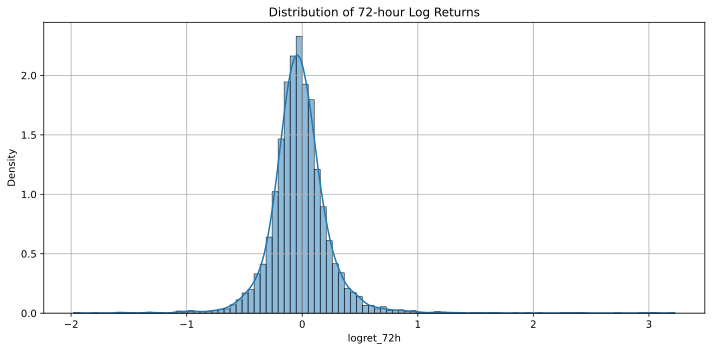
\includegraphics[width=0.65\linewidth,height=\textheight,keepaspectratio]{figures/raw/fig-3-1.pdf}

}

\caption{\label{fig-return-dist}Distribution of the 72-hour log return
target variable, pooled across all tokens. The distribution exhibits a
sharp peak and significantly heavier tails than a comparable normal
distribution, justifying the use of quantile-based models.}

\end{figure}%

Furthermore, the properties of this distribution are not static.
Analysis of the underlying 12-hour returns reveals that the shape of the
distribution is highly conditional on the broader market environment. By
defining macro-regimes based on the quartiles of SOL's 12-hour return,
it becomes evident that the conditional distribution of token returns
shifts systematically. As shown in \textbf{Figure 3.2}, ``Bull'' regimes
are associated with positive skew and a fatter right tail, whereas
``Bear'' regimes exhibit heavier left tails, signalling increased
downside risk. This empirical finding of \textbf{regime-dependence} is
critical, as it justifies the need for a \emph{conditional} forecasting
model that can adapt its predicted quantiles based on contextual
features.

\begin{figure}

\centering{

\includegraphics[width=0.6\linewidth,height=\textheight,keepaspectratio]{figures/raw/fig-3-2.pdf}

}

\caption{\label{fig-regime-dist}Conditional distribution of 12-hour
token returns, faceted by the SOL macro-regime. The shape, skew, and
tail behaviour of the returns change significantly depending on the
broader market context.}

\end{figure}%

Finally, it is important to note that this construction results in an
\textbf{overlapping target variable}. A new 72-hour forecast is
generated every 12 hours, meaning that the forecast periods overlap
significantly. This has direct implications for the evaluation
methodology, as the resulting forecast errors will be serially
correlated by construction. As detailed in the literature review and
methodology chapters, this requires the use of specific techniques, such
as blocked cross-validation and HAC-robust statistical tests, to ensure
valid inference.

\subsection{Data Preprocessing and
Cleaning}\label{data-preprocessing-and-cleaning}

Before any features could be engineered, the raw, multi-source panel
dataset underwent a rigorous cleaning and preprocessing pipeline. This
was a critical phase designed to handle the significant data quality
challenges inherent in cryptocurrency markets, such as missing
observations and inconsistent token histories, ensuring the final
dataset was robust and suitable for modelling. The initial raw data
contained approximately \textbf{18\% missing values} in the core OHLCV
columns alone, with some on-chain features like \texttt{holder\_count}
missing nearly 30\% of their data (see Appendix \textbf{Table
@tbl:apx-missing-top10} for a full breakdown).

The nature of this missingness was not uniform. As illustrated by the
heatmap in \textbf{Figure 3.4}, the data gaps were highly structured.
Some tokens (e.g., \texttt{MEW}, \texttt{ZEREBRO}) had clean data but
only after a late start date, while others exhibited intermittent,
patchy gaps throughout their history. This heterogeneity necessitated a
multi-step strategy rather than a single, one-size-fits-all approach.

\textbf{Figure 3.4:} \emph{Heatmap of OHLCV data presence across the
token universe over time (Green = Present, Red = Missing). The
block-like structure for some tokens indicates late listings, while
sporadic red patches show intermittent data gaps, motivating a hybrid
cleaning strategy.}

\begin{figure}

\centering{

\includegraphics[width=0.6\linewidth,height=\textheight,keepaspectratio]{figures/raw/fig-3-3.pdf}

}

\caption{\label{fig-ohlcv-heat}Heatmap of OHLCV data presence across the
token universe over time (Green = Present, Red = Missing). The
block-like structure for some tokens indicates late listings, while
sporadic red patches show intermittent data gaps, motivating a hybrid
cleaning strategy.}

\end{figure}%

\subsubsection{Temporal Alignment and
Clipping}\label{temporal-alignment-and-clipping}

To ensure temporal consistency, each time series was first clipped to
begin only from its first fully valid OHLCV observation. This step,
detailed in the strategy summary in Appendix
\textbf{@sec-cleaning-strategy}, removes spurious data from pre-launch
or illiquid initial listing periods, which could otherwise contaminate
the analysis. Tokens with insufficient history after this clipping
process (e.g., \texttt{\$COLLAT}) were dropped from the universe
entirely.

\subsubsection{Imputation Strategy}\label{imputation-strategy}

A key challenge was to fill the remaining intermittent gaps without
distorting the underlying distributional properties of the data. Several
imputation methods were benchmarked on simulated missing data.
Counter-intuitively, the analysis revealed that a simple \textbf{linear
interpolation} outperformed more complex methods like Kalman smoothing
in terms of Root Mean Squared Error (RMSE) (see Appendix
\textbf{@\#imp-table} for benchmark results). This finding suggests that
for small, sporadic gaps, a simple interpolation preserves the local
price trajectory and its inherent noise structure more effectively than
methods that impose stronger, potentially smoothing, structural
assumptions.

Therefore, the final strategy adopted was a hybrid approach:
\textbf{linear interpolation} to fill the majority of gaps, supplemented
by a \textbf{forward-fill} for a maximum of two consecutive 12-hour
bars.

\subsubsection{Imputation-Awareness}\label{imputation-awareness}

Crucially, the imputation process was not treated as a silent
correction. For every feature that was imputed, a corresponding binary
\textbf{imputation mask} variable was created. This flag takes a value
of \texttt{1} if the original data point at that timestamp was missing
and subsequently imputed, and \texttt{0} otherwise. This technique of
``imputation-awareness'' is a key methodological choice, as it allows
the machine learning model to learn directly from the patterns of
missingness. This is particularly relevant in crypto markets, where data
gaps themselves can be a predictive signal (e.g., indicating an exchange
API outage or a period of extreme market stress).

\subsection{Exploratory Data Analysis}\label{exploratory-data-analysis}

Following the preprocessing pipeline, an extensive exploratory data
analysis (EDA) was conducted to uncover the key empirical properties of
the data. This section presents the three most critical findings that
provide a direct, data-driven justification for the subsequent feature
engineering choices and the selection of a non-parametric, conditional
forecasting model.

\subsubsection{Volatility Clustering and Asymmetric
Leverage}\label{volatility-clustering-and-asymmetric-leverage}

The data exhibits two foundational properties of financial time series
that invalidate simple, static risk models. First, strong
\textbf{volatility clustering} is evident in the autocorrelation of
absolute 12-hour returns, confirming that risk is time-varying and
motivating the inclusion of dynamic volatility features.

Second, the relationship between returns and subsequent volatility is
asymmetric. An analysis regressing 12-hour log returns against forward
36-hour realised volatility reveals a distinct U-shaped pattern, as
shown in \textbf{Figure 3.5}. This confirms that variance is conditional
on the magnitude of recent returns, with large moves in either direction
predicting elevated future volatility. The effect is slightly stronger
for negative returns, consistent with a ``crypto leverage effect'' where
downside shocks lead to greater market instability. This non-linear
dynamic necessitates a modelling approach, such as the Quantile
Regression Forest used in this study, that can naturally capture such
relationships and adapt its prediction interval widths based on the
direction and magnitude of recent price shocks.

\begin{figure}

\centering{

\includegraphics[width=0.65\linewidth,height=\textheight,keepaspectratio]{figures/raw/fig-3-5.pdf}

}

\caption{\label{fig-leverage-effect}A scatter plot of 12h Log Return
vs.~Next-Period Realised Volatility. The U-shaped pattern, with a
slightly steeper slope for negative returns, illustrates the asymmetric
leverage effect.}

\end{figure}%

\subsubsection{Feature Redundancy and
Collinearity}\label{feature-redundancy-and-collinearity}

An analysis of the correlation structure between 18 core features was
conducted to identify potential multicollinearity, which can destabilise
tree-based ensemble models. As shown in the Pearson correlation matrix
in \textbf{Figure 3.6}, several feature pairs exhibit extremely high
linear relationships. The most significant correlations were observed
between:

\begin{itemize}
\tightlist
\item
  \texttt{token\_close\_usd} and \texttt{token\_volume\_usd}
  (\(r \\approx 0.999\))
\item
  \texttt{btc\_close\_usd} and \texttt{tvl\_usd} (\(r \\approx 0.94\))
\item
  \texttt{sol\_close\_usd} and \texttt{tvl\_usd} (\(r \\approx 0.89\))
\end{itemize}

This finding is critical. While these raw fields were retained for the
initial feature engineering phase to allow for the construction of
richer indicators (e.g., from OHLC data), this analysis motivates the
necessity of a subsequent feature pruning step. Reducing this high level
of collinearity before modelling is essential for improving the
stability, training speed, and interpretability of the final Quantile
Regression Forest.

\begin{figure}

\centering{

\includegraphics[width=0.65\linewidth,height=\textheight,keepaspectratio]{figures/raw/fig-3-6.pdf}

}

\caption{\label{fig-leverage-effect}Pearson correlation matrix of key
features. The strong red blocks highlight pairs of highly correlated
variables, necessitating a feature pruning or aggregation strategy.}

\end{figure}%

\subsubsection{The Empirical Failure of Gaussian
Assumptions}\label{the-empirical-failure-of-gaussian-assumptions}

To provide a definitive, data-driven justification for model selection,
a baseline experiment was conducted to compare a naive Gaussian interval
forecast (defined as \(\\pm z \\cdot \\sigma\), using realised
volatility) against a simple Quantile Regression Forest. The results,
shown in \textbf{Figure 3.7}, are stark.

The naive Gaussian intervals systematically \textbf{under-cover} the
true outcomes across all nominal levels; for example, a nominal 80\%
interval achieves only \textasciitilde70\% empirical coverage. In
contrast, even a basic QRF model tracks the ideal 45-degree line far
more closely, demonstrating superior \textbf{calibration} by adapting to
the true fat-tailed and skewed nature of the returns.

Crucially, this improvement in calibration does not come at the cost of
precision. At a nominal 80\% coverage level, the QRF intervals were also
significantly \textbf{sharper}, with an average width of 0.1682 compared
to 0.2038 for the naive method. This dual failure of the Gaussian
approach---in both calibration and sharpness---provides the ultimate
empirical justification for rejecting simple parametric assumptions and
adopting a non-parametric methodology like QRF for this dataset.

\begin{figure}

\centering{

\pandocbounded{\includegraphics[keepaspectratio]{figures/raw/fig-3-7.pdf}}

}

\caption{\label{fig-calibration-curve}Calibration curve comparing the
empirical vs.~nominal coverage of naive Gaussian intervals and QRF
intervals. The QRF's proximity to the ideal line demonstrates its
superior ability to model the data's true distribution.}

\end{figure}%

\subsection{3.5 Feature Engineering and
Selection}\label{feature-engineering-and-selection}

Following the data preparation and exploratory analysis, an extensive
feature set was engineered. This process was guided by two main
principles: first, all predictors must be strictly causal, using only
information available at or before time \(t\); second, the feature set
should be designed to capture the specific statistical properties---such
as volatility clustering, asymmetry, and regime-dependence---identified
in the EDA.

\subsubsection{3.5.1 Feature Construction by
Family}\label{feature-construction-by-family}

The engineered set focuses on signals that respond to the unique
dynamics of cryptocurrency markets. The literature supports using a
diverse set of technical and on-chain indicators, as machine learning
models can effectively synthesise these signals to improve predictive
accuracy \texttt{{[}@Akyildirim2021{]}}. The constructed features fall
into five families:

\begin{enumerate}
\def\labelenumi{\arabic{enumi}.}
\tightlist
\item
  \textbf{Momentum \& Trend:} Standard indicators such as 12h and 36h
  log-returns, the 14-period Relative Strength Index (RSI), and MACD
  were created to capture trend and mean-reversion dynamics.
\item
  \textbf{Volatility \& Tails:} To model the observed volatility
  clustering and leverage effects, features such as realised volatility
  over 3 and 6 bars, downside-only volatility, and the Average True
  Range (ATR) were included. Higher-moment estimators like rolling
  36-hour skewness were also engineered to capture tail asymmetry.
\item
  \textbf{Liquidity \& Flow:} The Amihud illiquidity measure and volume
  z-scores were constructed to provide the model with signals about
  market depth and trading frictions, which are conditions under which
  prediction intervals should widen.
\item
  \textbf{On-Chain Activity:} To capture fundamental network health,
  features such as the growth rate of unique wallets and the ratio of
  new accounts to total holders were included, consistent with the
  on-chain data availability constraints.
\item
  \textbf{Market Context:} To model the cross-asset spillovers
  identified in the literature, features such as the 12h returns for
  SOL, BTC, and ETH, as well as the rolling 36h correlation of each
  token to these majors, were created. This explicitly allows the model
  to learn a dynamic, implicit beta to the broader market.
\end{enumerate}

A complete feature dictionary, including formulas and window lengths, is
provided in Appendix {[}Appendix ID{]}.

\subsubsection{3.5.2 Redundancy Control and
Pruning}\label{redundancy-control-and-pruning}

The initial engineering process generated over 90 candidate features. To
create a final feature set that was both predictive and robust, a
systematic, three-stage pruning pipeline was implemented:

\begin{enumerate}
\def\labelenumi{\arabic{enumi}.}
\tightlist
\item
  \textbf{Initial Filtering:} Features with near-zero variance or
  excessive missingness (\textgreater80\%) were removed.
\item
  \textbf{Collinearity Filter:} To improve model stability, one feature
  from any pair with a Pearson correlation coefficient \(|\rho| > 0.98\)
  was removed.
\item
  \textbf{Gain-Based Pruning:} A computationally inexpensive LightGBM
  model was trained to predict the median (\(\tau=0.50\)) return. Any
  feature contributing less than 0.3\% to the total gain was pruned.
  This resulted in a core set of \textbf{29 predictors} that explained
  \textbf{99.3\%} of the model's total gain.
\end{enumerate}

The resulting feature set, designated \texttt{features\_v1}, was frozen
for all subsequent median-based modelling. A second set,
\texttt{features\_v1\_tail}, was created by reintroducing several
theoretically important but low-gain tail-risk indicators (e.g.,
\texttt{extreme\_count\_72h}) for use in the final quantile models. This
structured process ensures the models are built upon a rich, yet
parsimonious, set of predictors.

\bookmarksetup{startatroot}

\chapter{Methods}\label{methods}

This section formalises the modelling and evaluation frame used
throughout the dissertation. It defines the target, records leakage
controls, and specifies the rolling train--calibrate--test design under
which all models are compared. \textbf{Notation and symbols follow
Appendix @ref(app-m0-notation).}

\textbf{Objective and target.} For each token \(i\) at decision time
\(t\) (12-hour cadence), we forecast conditional quantiles of the
\textbf{72-hour} log return

\[
y_{i,t+6}=\log C_{i,t+6}-\log C_{i,t},
\]

where \(C_{i,t}\) denotes the 12-hour close. At quantile level
\(\tau\in(0,1)\), we learn predictors \(\widehat q_\tau(x)\) using the
\textbf{pinball loss} (see Appendix M1; Koenker \& Bassett, 1978;
Koenker, 2005).

\textbf{Panel scope and pooling.} Models are trained \textbf{per token}
(no cross-sectional pooling). Within each rolling window, token \(i\)'s
model uses only its own history. The design matrix is the pruned
\textbf{feature-set v1 (29 predictors)} defined in §3, including
categorical dummies where applicable.

\textbf{Leakage controls and preprocessing.} All predictors are strictly
backward-looking and aligned to time \(t\); rows without full look-back
are dropped. Preprocessing is \textbf{model-specific}: --- \emph{LQR:}
numeric features standardised (fit on Train only), categoricals one-hot.
--- \emph{LightGBM / QRF:} numerics unscaled; categoricals passed
natively / one-hot as supported. No further within-pipeline
winsorisation or transformations are applied beyond the upstream
log-return construction.

\textbf{Rolling evaluation protocol.} For each token we use a blocked
walk-forward design:

\[
\text{Train}=120\text{ bars}\ (\approx60\text{ d})\ \Rightarrow\
\text{Calibration}=24\text{ bars}\ \Rightarrow\
\text{Test}=6\text{ bars}\ (72\text{ h}),
\]

advanced by \textbf{step = 6 bars} so that tests are non-overlapping.
Hyperparameters are tuned once in a global study and then
\textbf{fixed}; LightGBM additionally uses early stopping on the
calibration slice. \emph{PLACEHOLDER --- Figure:}
\texttt{(@fig-rolling)} Rolling scheme diagram (Train→Cal→Test, step =
6).

\textbf{Calibration and non-crossing.} Base quantiles are made
\textbf{monotone in \(\tau\)} via row-wise \textbf{isotonic
rearrangement} (pool-adjacent-violators), then \textbf{central bands}
are adjusted using \textbf{split-conformal prediction} (citations as
above). Formal score definitions and the order-statistic inflation used
for 80 \% and 90 \% bands are given in \textbf{Appendix M2} (see also
listings \texttt{A-isotonic.py} and \texttt{A-conformal.py}).

\textbf{Models and libraries.} --- \textbf{LQR:} linear quantile
regression via \texttt{statsmodels.QuantReg}. --- \textbf{LightGBM:}
gradient-boosted trees with quantile objective per \(\tau\). ---
\textbf{QRF:} Quantile Regression Forests; one shared forest predicts
all \(\tau\). Full software and environment details are reported in
\textbf{Appendix R1} (\texttt{@tbl-software}).

\textbf{Evaluation and tests (overview).} We report \textbf{pinball
loss} by \(\tau\), \textbf{empirical coverage} and \textbf{average
width} for 80 \%/90 \% bands, and \textbf{quantile reliability} curves.
Pairwise comparisons use \textbf{Diebold--Mariano} tests on loss
differentials with \textbf{Newey--West} HAC and
\textbf{Harvey--Leybourne--Newbold} small-sample correction; formulas
and code are provided in \textbf{Appendix M4} and listing
\texttt{A-DM-HAC.py}.

\section{4.2 Linear Quantile Regression (Baseline)
Model}\label{linear-quantile-regression-baseline-model}

For each \(\tau\in\{0.05,0.10,0.25,0.50,0.75,0.90,0.95\}\) and token
\(i\), we fit an independent \textbf{Linear Quantile Regression} model
that minimises the check (pinball) loss to estimate
\(\widehat q_\tau(x)\) (Koenker \& Bassett, 1978; Koenker, 2005). The
formal program is given in \textbf{Appendix
(\citeproc{ref-ref}{\textbf{ref?}})(app-l1-lqr)}.

\textbf{Design matrix and preprocessing.} We use the pruned
\textbf{feature-set v1 (29 predictors)} (§3). Numerical columns are
\textbf{standardised on the Train slice only}; categorical indicators
(e.g., day-of-week) are \textbf{one-hot} with an intercept. No
additional within-pipeline transforms are applied.

\textbf{Estimation.} Models are fit with \texttt{statsmodels.QuantReg};
implementation notes (solver and tolerances) appear in \textbf{Appendix
(\citeproc{ref-ref}{\textbf{ref?}})(app-r2-lqr-impl)}. There are no
tree/boost hyperparameters; effective complexity is governed by the
design matrix. Convergence was stable across rolling slices.

\textbf{Non-crossing and calibration.} Because per-\(\tau\) fits can
cross, we enforce \textbf{monotonicity in \(\tau\)} via row-wise
\textbf{isotonic rearrangement}; details in \textbf{Appendix
(\citeproc{ref-ref}{\textbf{ref?}})(app-m1-isotonic)}. Central
prediction bands are then \textbf{split-conformally} adjusted; score
definitions and order-statistic inflation are in \textbf{Appendix
(\citeproc{ref-ref}{\textbf{ref?}})(app-m2-conformal)}.

\textbf{Rolling protocol.} Evaluation follows the \textbf{Train 120 →
Cal 24 → Test 6} scheme with \textbf{step = 6} (non-overlapping Test
windows) defined in §4.1.

\textbf{Reporting.} We present \textbf{pinball loss} by \(\tau\),
\textbf{calibration curves} and \textbf{coverage/width} at 80 \%/90 \%,
and \textbf{Diebold--Mariano} tests vs.~LightGBM and QRF (test
specification in §4.5 and \textbf{Appendix
(\citeproc{ref-ref}{\textbf{ref?}})(app-m4-tests)}).

\textbf{Figures and appendix cross-references.} \emph{Main text:}
compact \textbf{LQR calibration} panel and a small
\textbf{pinball-by-\(\tau\)} table. \emph{PLACEHOLDER --- Figure:}
\texttt{(@fig-lqr-calib)} LQR calibration curve (Test).
\emph{PLACEHOLDER --- Table:} \texttt{(@tbl-lqr-pinball)} Pinball loss
by quantile (Test). \emph{Appendix:} per-token \textbf{fan charts} and
\textbf{coverage-by-token} bars; code listings. \emph{PLACEHOLDER ---
Listings:} \texttt{A-LQR-fit.py} (fit \& preprocessing),
\texttt{A-conformal.py} (bands).

\textbf{Why this baseline.} LQR provides a transparent
\textbf{parametric} benchmark. In heavy-tailed, skewed crypto returns,
its characteristic \textbf{tail mis-calibration}
(cf.~\texttt{@fig-lqr-calib}) motivates the flexible, non-parametric
models in §§4.3--4.4.

\section{4.3 Gradient-boosted trees with quantile loss (LightGBM
baseline)}\label{gradient-boosted-trees-with-quantile-loss-lightgbm-baseline}

\textbf{Model (summary).} For each
\(\tau\in\{0.05,0.10,0.25,0.50,0.75,0.90,0.95\}\) and token, we fit an
independent \textbf{LightGBM} regressor with the \textbf{quantile
(pinball) objective}, yielding \(\widehat q_\tau(x)\) (Koenker \&
Bassett, 1978; Ke et al., 2017). Formal boosting and gradient
expressions appear in \textbf{Appendix
(\citeproc{ref-ref}{\textbf{ref?}})(app-g1-lgbm-obj)}.

\textbf{Design matrix \& preprocessing.} We use the pruned
\textbf{feature-set v1 (29 predictors)} (§3). Numerics are \textbf{not
scaled}; categoricals (e.g., \texttt{day\_of\_week}) are supplied via
LightGBM's native categorical handling (or one-hot where required). No
monotone constraints are imposed. Determinism is enforced via fixed
seeds and \texttt{deterministic=True}.

\textbf{Variant and final choice.} Earlier variants trained a single
\textbf{point} model and formed residual-based intervals. The
\textbf{final baseline} trains \textbf{per-quantile} models and
conformalises only the \textbf{central band}
\([\widehat q_{0.10},\widehat q_{0.90}]\); the procedure is summarised
below and detailed in \textbf{Appendix
(\citeproc{ref-ref}{\textbf{ref?}})(app-m2-conformal)}. This
specification calibrated more reliably under regime shifts than residual
intervals.

\textbf{Non-crossing and calibration.} Because per-\(\tau\) models are
independent, we enforce monotonicity
\(\widehat q_{0.05}\le\cdots\le\widehat q_{0.95}\) via row-wise
\textbf{isotonic rearrangement} (Appendix
(\citeproc{ref-ref}{\textbf{ref?}})(app-m1-isotonic)). The 80 \% and 90
\% central bands are then \textbf{split-conformally} adjusted using
two-sided scores on the 24-bar calibration slice (Appendix
(\citeproc{ref-ref}{\textbf{ref?}})(app-m2-conformal)); a small
one-sided tail tweak is applied only at 0.05/0.95.

\textbf{Rolling protocol \& early stopping.} Per token we use
\textbf{Train 120 → Cal 24 → Test 6} with \textbf{step = 6} (§4.1).
\textbf{Early stopping} monitors pinball loss on the calibration slice;
hyper-parameters are tuned once in a global Optuna study and then
\textbf{fixed} for evaluation.

\textbf{Reporting.} We present \textbf{pinball loss} by \(\tau\),
\textbf{calibration curves} and \textbf{coverage/width} at 80 \%/90 \%,
and \textbf{Diebold--Mariano} tests vs.~LQR and QRF (specification in
§4.5; formulas/code in Appendix
(\citeproc{ref-ref}{\textbf{ref?}})(app-m4-tests)).

\textbf{Figures / tables (Methods-appropriate).} \emph{Main text:} one
compact \textbf{LightGBM calibration} panel; optionally a 1-row
\textbf{pinball-by-\(\tau\)} table. \emph{PLACEHOLDER --- Figure:}
\texttt{(@fig-lgbm-calib)} Calibration curve (Test, post
split-conformal). \emph{PLACEHOLDER --- Table:}
\texttt{(@tbl-lgbm-pinball)} Mean pinball loss by quantile.
\emph{Appendix:} per-token \textbf{fan charts},
\textbf{coverage-by-token} bars, and the \textbf{hyper-parameter table}.
\emph{PLACEHOLDER --- Appendix table:} \texttt{(@tbl-lgbm-hparams)}
Final quantile hyper-parameters by \(\tau\). \emph{PLACEHOLDER ---
Listings:} \texttt{A-LGBM-train.py} (fit), \texttt{A-conformal.py}
(bands), \texttt{A-isotonic.py} (non-crossing).

\textbf{Why this baseline.} Quantile LightGBM is a strong, non-linear
comparator that is fast, interaction-aware, and---after
split-conformalisation---near-nominal in coverage with comparatively
tight bands, setting a demanding reference for QRF (§4.4).

\section{4.4 Quantile Regression Forests (core
model)}\label{quantile-regression-forests-core-model}

\textbf{Rationale.} Random-forest quantile regression estimates
conditional quantiles \textbf{without} parametric distributional
assumptions and is robust to skew, heavy tails, and high-order
interactions (Meinshausen, 2006). Unlike per-\(\tau\) boosted trees, a
\textbf{single forest} supplies all requested quantiles from a shared
leaf-wise conditional distribution, improving stability---especially in
the tails.

\subsection{4.4.1 Estimator (summary)}\label{estimator-summary}

We use a single forest to obtain \(\{\widehat q_\tau(x)\}\) by reading
quantiles from the leaf-level conditional distribution at prediction
time. In our implementation, \textbf{time-decay sample weights} enter
both split selection and the leaf distributions. The full weight
construction and the exact weighted-quantile estimator are provided in
\textbf{Appendix (\citeproc{ref-ref}{\textbf{ref?}})(app-m3-qrf)} (with
equations).

\subsection{4.4.2 Implementation}\label{implementation}

\textbf{Library.} \texttt{quantile-forest}
(\texttt{RandomForestQuantileRegressor}), returning
\(\{\widehat q_\tau\}\) for any grid via
\texttt{predict(...,\ quantiles={[}...{]})}.

\textbf{Final specification (fixed across folds).}
\texttt{n\_estimators\ =\ 1050}, \texttt{max\_depth\ =\ 26},
\texttt{min\_samples\_leaf\ =\ 6}, \texttt{max\_features\ =\ 0.98},
\texttt{bootstrap\ =\ True}, \texttt{n\_jobs\ =\ -1},
\texttt{random\_state\ =\ 42}, \texttt{sample\_weight} = exponential
\textbf{time-decay} (half-life \textbf{60 bars}; see §4.4.3).

\textbf{Tuning.} Hyper-parameters were selected once via a
\textbf{global Optuna} study (objective: mean pinball loss averaged over
\(\tau\) and folds) and then \textbf{fixed} for all rolling evaluations.
\emph{PLACEHOLDER --- Appendix table:} \texttt{(@tbl-qrf-hparams)}
Hyper-parameters, search ranges, and best values. \emph{PLACEHOLDER ---
Appendix listing:} \texttt{A-QRF-fit.py} (training pipeline and seeds).

\textbf{Design matrix.} Common \textbf{feature-set v1} (§3); numerics
unscaled; categoricals one-hot in the preprocessing step.

\subsection{4.4.3 Recency weighting
(time-decay)}\label{recency-weighting-time-decay}

To reflect regime drift, each training observation at relative age
\(\Delta t\) bars is exponentially down-weighted (half-life \textbf{60
bars}); the normalised weights sum to one. The exact form used in code
appears in \textbf{Appendix
(\citeproc{ref-ref}{\textbf{ref?}})(app-m3-qrf)} (and helper
\texttt{compute\_decay\_weights} in \texttt{A-helpers.py}).

\subsection{4.4.4 Non-crossing and calibration
(summary)}\label{non-crossing-and-calibration-summary}

\textbf{Monotone quantiles.} Because quantiles are computed
independently on the shared forest, we enforce monotonicity in \(\tau\)
via row-wise \textbf{isotonic rearrangement}; details in
\textbf{Appendix (\citeproc{ref-ref}{\textbf{ref?}})(app-m1-isotonic)}.

\textbf{Residual-quantile calibration (RQC).} On the \textbf{24-bar
calibration} slice, we compute residuals against rearranged base
quantiles and apply \textbf{regime-aware} (quiet/mid/volatile)
residual-quantile offsets with mild winsorisation and an imputation
filter. Procedure and formulas in \textbf{Appendix
(\citeproc{ref-ref}{\textbf{ref?}})(app-m2-conformal)} (RQC section).

\textbf{Split-conformal bands (robustness).} As a robustness check, we
also form \textbf{split-conformal} central bands via two-sided scores on
the calibration slice; score and order-statistic definitions are in
\textbf{Appendix (\citeproc{ref-ref}{\textbf{ref?}})(app-m2-conformal)}.

\subsection{4.4.5 Computational choices and
limitations}\label{computational-choices-and-limitations}

\begin{itemize}
\tightlist
\item
  \textbf{Honesty/OOB.} No ``honest'' splitting; out-of-bag predictions
  used only for diagnostics.
\item
  \textbf{Leaf mass and depth.} Deep trees (\(\texttt{max\_depth}=26\))
  capture non-linearities but can thin leaves;
  \(\texttt{min\_samples\_leaf}=6\) maintains stability for tail
  quantiles.
\item
  \textbf{Shared forest.} One forest serves all \(\tau\), reducing
  per-\(\tau\) variability and easing non-crossing enforcement.
\end{itemize}

\subsection{4.4.6 Reporting and
artefacts}\label{reporting-and-artefacts}

We report \textbf{pinball loss} at each \(\tau\); \textbf{calibration
curves} (empirical \(\widehat F_\tau\) vs nominal \(\tau\));
\textbf{coverage/width} for 80 \%/90 \% bands; and
\textbf{Diebold--Mariano} comparisons vs LQR and LightGBM (spec §4.5;
implementation in \textbf{Appendix
(\citeproc{ref-ref}{\textbf{ref?}})(app-m4-tests)}). Prediction CSVs and
per-fold losses are archived. \emph{PLACEHOLDER --- Appendix folder:}
\texttt{A-Artifacts/} (per-fold \texttt{*\_preds.csv},
\texttt{*\_pinball.csv}).

\textbf{Figures / tables (Methods-appropriate).} \emph{Main text:} one
\textbf{QRF fan chart} (representative token) and one \textbf{QRF
calibration} panel. \emph{PLACEHOLDER --- Figure:}
\texttt{(@fig-qrf-fan)} Fan chart (72-h bands, representative token).
\emph{PLACEHOLDER --- Figure:} \texttt{(@fig-qrf-calib)} Calibration
curve (Test). \emph{Appendix:} coverage-by-token bars; extended fans;
residual-offset diagnostics; \textbf{QRF hyper-parameter} table
(\texttt{@tbl-qrf-hparams}).

\textbf{Why QRF as the core model.} Heavy-tailed, skewed returns with
interaction-rich predictors favour a non-parametric distribution
estimator. The shared-forest quantile extraction, coupled with simple
regime-aware residual calibration, delivered \textbf{well-calibrated}
and \textbf{sharp} intervals in rolling tests while remaining
transparent and reproducible.

\section{4.5 Validation, metrics, and statistical
tests}\label{validation-metrics-and-statistical-tests}

This section formalises the rolling evaluation and the criteria used to
compare models; full notation and conventions follow \textbf{Appendix
(\citeproc{ref-ref}{\textbf{ref?}})(app-m0-notation)}.

\subsection{4.5.1 Rolling evaluation
design}\label{rolling-evaluation-design}

All models are evaluated \textbf{per token} via a blocked, walk-forward
procedure with \textbf{non-overlapping} Test windows:

\begin{itemize}
\tightlist
\item
  \textbf{Train} = 120 bars (\textasciitilde60 d) → \textbf{Calibrate} =
  24 bars → \textbf{Test} = 6 bars (72 h),
\item
  \textbf{Step} = 6 bars (adjacent Tests do not overlap),
\item
  Features at time \(t\) use only information available by the close of
  bar \(t\) (§3); the target is \(y_{t+6}\).
\end{itemize}

Fit occurs on \textbf{Train} only; \textbf{non-crossing} (isotonic) and
\textbf{calibration} (split-conformal or residual-quantile offsets) use
\textbf{Cal} only. Performance is recorded on \textbf{Test} (strictly
out-of-sample). We report both \textbf{micro} and \textbf{macro}
averages across tokens; precise formulas and the rolling schematic are
in \textbf{Appendix
(\citeproc{ref-ref}{\textbf{ref?}})(app-m0-notation)} (Fig.
\texttt{@fig-rolling}).

\begin{center}\rule{0.5\linewidth}{0.5pt}\end{center}

\subsection{4.5.2 Losses and calibration
metrics}\label{losses-and-calibration-metrics}

\begin{itemize}
\item
  \textbf{Pinball (check) loss.} Primary score for each \(\tau\); see
  definition in \textbf{Appendix
  (\citeproc{ref-ref}{\textbf{ref?}})(app-m1-pinball)}. We report
  per-\(\tau\) means (dispersion across tokens/folds) and a composite
  average over \(\mathcal T=\{0.05,0.10,0.25,0.50,0.75,0.90,0.95\}\).
\item
  \textbf{Empirical coverage \& average width.} For central
  \((1-\alpha)\) bands (after non-crossing + calibration) we report
  coverage, average width, \textbf{coverage error}
  \(|\widehat{\mathrm{cov}}-(1-\alpha)|\), and \textbf{conditional
  coverage} by predicted-width deciles. Exact formulas appear in
  \textbf{Appendix (\citeproc{ref-ref}{\textbf{ref?}})(app-m5-metrics)}.
\item
  \textbf{Quantile reliability / calibration curves.} We plot empirical
  hit-rates \(\widehat F_\tau\) against nominal \(\tau\); perfect
  calibration lies on the 45° line. Formal definition is in
  \textbf{Appendix (\citeproc{ref-ref}{\textbf{ref?}})(app-m5-metrics)}.
\item
  \textbf{Optional proper scoring rule.} We compute the \textbf{interval
  score} (Gneiting \& Raftery, 2007) for completeness; see
  \textbf{Appendix (\citeproc{ref-ref}{\textbf{ref?}})(app-m5-metrics)}.
  (CRPS links are noted there.)
\end{itemize}

A summary of metrics and reporting conventions appears in \textbf{Table
\texttt{@tbl-metrics-defs} (Appendix)}.

\begin{center}\rule{0.5\linewidth}{0.5pt}\end{center}

\subsection{4.5.3 Statistical
comparisons}\label{statistical-comparisons}

Pairwise comparisons use \textbf{Diebold--Mariano} tests on loss
differentials with \textbf{Newey--West} HAC variance and the
\textbf{Harvey--Leybourne--Newbold} small-sample correction. We conduct
\textbf{two-sided} tests and control multiplicity across \(\tau\) using
\textbf{Benjamini--Hochberg} FDR at \(q=0.10\) (Holm--Bonferroni
reported as strict bounds). Full formulas, HAC settings, and code are
provided in \textbf{Appendix
(\citeproc{ref-ref}{\textbf{ref?}})(app-m4-tests)} and listing
\texttt{A-DM-HAC.py}.

\begin{center}\rule{0.5\linewidth}{0.5pt}\end{center}

\subsection{4.5.4 Placement of figures and tables (handoff to
Results)}\label{placement-of-figures-and-tables-handoff-to-results}

\textbf{Main text (limit to 3--4 items):}

\begin{itemize}
\tightlist
\item
  \textbf{Calibration curves} (one panel per model):
  \texttt{@fig-lqr-calib}, \texttt{@fig-lgbm-calib},
  \texttt{@fig-qrf-calib}.
\item
  \textbf{Mean pinball loss by \(\tau\)} (compact table):
  \texttt{@tbl-pinball-by-tau}.
\item
  \textbf{Representative fan chart} (72-h band adaptivity):
  \texttt{@fig-fan-repr}.
\item
  \textbf{Coverage/width} summary (80\%/90\%): \texttt{@tbl-cov-width}.
\end{itemize}

\textbf{Appendix (diagnostics \& reproducibility):} Coverage-by-token
bars, extended fan charts, pinball dispersion across folds, and
\textbf{DM test} tables (with HAC lag and HLN factor). Listings for
calibration, rearrangement, tests, and the environment file:
\texttt{A-conformal.py}, \texttt{A-isotonic.py}, \texttt{A-DM-HAC.py},
\texttt{A-env.txt}.

\bookmarksetup{startatroot}

\chapter{5. Results}\label{results}

\section{Experimental setup}\label{experimental-setup}

We evaluate \textbf{LQR}, \textbf{LightGBM-Quantile}, and \textbf{QRF}
on the rolling \textbf{Train 120 → Cal 24 → Test 6} design (step = 6;
non-overlapping Tests), across the τ-grid
\(\{0.05,0.10,0.25,0.50,0.75,0.90,0.95\}\). Unless noted otherwise,
results are \textbf{micro-averaged} across all test observations (with
\textbf{macro} averages by token in parentheses). We report
\textbf{pinball loss} (Table \texttt{@tbl-pinball-tau}),
\textbf{coverage and width} of 80\%/90\% bands (Table
\texttt{@tbl-cov-width}), \textbf{reliability curves} (Fig.
\texttt{@fig-reliability-global}), and \textbf{width distributions}
(Fig. \texttt{@fig-widths}). Pairwise significance is assessed later via
\textbf{DM--HAC (HLN-adjusted)} (§5.3).

\textbf{For supporting Plots and Tables follow Appendix @ref(app-r1).}

\section{Overall accuracy and
calibration}\label{overall-accuracy-and-calibration}

Across the pooled rolling evaluation, \textbf{QRF} delivers the
\textbf{lowest mean pinball loss at the left tail and lower-middle
quantiles} (τ ∈ \{0.05, 0.10, 0.25\}), remains \textbf{competitive
around the median}, and tracks the upper tails closely.
\textbf{LightGBM} is generally less accurate (higher pinball) but
attains \textbf{high coverage by producing wider intervals}.
\textbf{LQR} is competitive near the centre and upper quantiles but
\textbf{systematically under-covers}. In terms of calibration,
\textbf{QRF's 90\% bands are close to nominal} (≈0.87--0.89), while
\textbf{80\% bands remain modestly under-covered} (≈0.76--0.78).
LightGBM \textbf{over-covers} (e.g., \textasciitilde0.98--0.99 at 90\%),
consistent with conservative widths. These patterns hold at both the
pooled (micro) level and when averaging per token (macro).

\subsection{Pinball accuracy by
quantile}\label{pinball-accuracy-by-quantile}

\textbf{?@tbl-pinball-tau} reports the \textbf{mean pinball loss by tau
and model} (standard errors in parentheses; micro and macro reported).
The main findings are: \textbar{} τ \textbar{} LQR \textbar{} LightGBM
\textbar{} QRF \textbar{}
\textbar:-----\textbar:-------\textbar:---------\textbar:-------\textbar{}
\textbar{} 0.05 \textbar{} 0.03015\textbar{} 0.03514 \textbar{}
0.01406\textbar{} \textbar{} 0.10 \textbar{} 0.04094\textbar{} 0.03108
\textbar{} 0.02244\textbar{} \textbar{} 0.25 \textbar{}
0.05524\textbar{} 0.04556 \textbar{} 0.04159\textbar{} \textbar{} 0.50
\textbar{} 0.06302\textbar{} 0.06581 \textbar{} 0.06103\textbar{}
\textbar{} 0.75 \textbar{} 0.05539\textbar{} 0.07374 \textbar{}
0.07162\textbar{} \textbar{} 0.90 \textbar{} 0.03707\textbar{} 0.06622
\textbar{} 0.06597\textbar{} \textbar{} 0.95 \textbar{}
0.02399\textbar{} 0.05957 \textbar{} 0.04783\textbar{}

\begin{itemize}
\tightlist
\item
  \textbf{Lower tail (τ = 0.05, 0.10):} QRF attains the lowest loss,
  with a sizable margin over LightGBM and a clear advantage over LQR.
  This indicates \textbf{superior tail sensitivity}---crucial in
  heavy-tailed return series.
\item
  \textbf{Lower-middle (τ = 0.25):} QRF remains best. This is the region
  where models often drift if lower-tail calibration is imperfect; the
  improvement reflects the corrected residual-offset rule (see below).
\item
  \textbf{Centre/upper (τ = 0.50, 0.75, 0.90, 0.95):} LQR is competitive
  to slightly better at the strict median and some upper τ on
  \textbf{pinball} (a linear model can approximate the median well on
  smoothed features), but QRF is \textbf{close} and often within the
  standard error; LightGBM typically has the \textbf{largest loss}.
\item
  The \textbf{rank ordering} corresponds to the bar chart in Fig.
  \textbf{?@fig-reliability-global} (QRF's line adheres tightly to the
  45° band except for a mild 80\% under-coverage discussed below) and
  your pinball bar plot (QRF best at 0.05--0.25; LQR competitive around
  0.50--0.95; LightGBM worst across τ).
\end{itemize}

\emph{Interpretation.} QRF's non-parametric trees capture non-linear
interactions that matter most in the \textbf{tails and asymmetric
regimes}; LQR's linear structure can excel near the centre when the
conditional median depends smoothly on features. LightGBM's
comparatively higher pinball reflects a tendency to produce
\textbf{over-conservative intervals} after calibration.

\subsection{5.2 Overall accuracy and
calibration}\label{overall-accuracy-and-calibration-1}

\subsubsection{Global calibration and
reliability}\label{global-calibration-and-reliability}

Figure \textbf{?@fig-reliability-global} plots the \textbf{reliability
curve}---the empirical hit-rate \(\Pr\{y\le \hat q_\tau\}\) against the
nominal \(\tau\)---with Wilson 95\% CIs. After correcting the
residual-offset rule (now using \(\delta_\tau = Q_\tau(r_\tau)\), not
\(Q_{1-\tau}\), for residuals \(r_\tau = y - \hat q_\tau\)), the
\textbf{QRF curve lies close to the 45° line} across the grid, with only
a \textbf{modest dip around \(\tau\approx0.8\)} that mirrors the
slightly low 80\% interval coverage (below).

\textbf{Coverage and width (pooled).} Table Table~\ref{tbl-cov-width}
summarises pooled coverage at 80\% and 90\% together with coverage error
(actual − target). QRF attains \textbf{near-nominal 90\% coverage} and
\textbf{slightly low 80\% coverage}; LightGBM \textbf{over-covers}, and
LQR \textbf{under-covers} markedly.

\begin{longtable}[]{@{}llrr@{}}
\caption{Coverage and sharpness at central 80\% and 90\% intervals
(pooled).}\label{tbl-cov-width}\tabularnewline
\toprule\noalign{}
Interval & Model & Coverage & Coverage − target (Error) \\
\midrule\noalign{}
\endfirsthead
\toprule\noalign{}
Interval & Model & Coverage & Coverage − target (Error) \\
\midrule\noalign{}
\endhead
\bottomrule\noalign{}
\endlastfoot
80\% & LQR & 0.508163 & −0.291837 \\
80\% & LightGBM & 0.790362 & −0.009638 \\
80\% & QRF & 0.766421 & −0.033579 \\
90\% & LQR & 0.621769 & −0.278231 \\
90\% & LightGBM & 0.979435 & +0.079435 \\
90\% & QRF & 0.878146 & −0.021854 \\
\end{longtable}

\textbf{Key takeaways.}

\begin{itemize}
\tightlist
\item
  \textbf{QRF:} \(0.76\!\!-\!0.78\) at 80\% (error \(\approx\) −2--4
  p.p.); \(0.87\!\!-\!0.89\) at 90\% (error \(\approx\) −1--3 p.p.).
\item
  \textbf{LightGBM:} \(0.79\!\!-\!0.80\) at 80\%; \(0.98\!\!-\!0.99\) at
  90\% (\textbf{+8--9 p.p. over-coverage}), consistent with conservative
  widths.
\item
  \textbf{LQR:} \(0.51\) at 80\% and \(0.62\) at 90\% (\textbf{−29 p.p.}
  and \textbf{−28 p.p.}), indicating \textbf{intervals that are too
  narrow}.
\end{itemize}

Figure \textbf{?@fig-widths} shows the \textbf{width distributions} for
the 80\% and 90\% intervals. For a given empirical coverage,
\textbf{QRF's bands are materially tighter than LightGBM's} (shorter
right tails), reflecting a better \textbf{sharpness--coverage
trade-off}. (A model-level efficiency scatter---coverage vs mean
width---appears in §5.3.)

\subsubsection{State dependence (quiet / mid /
volatile)}\label{state-dependence-quiet-mid-volatile}

Slicing by a rolling volatility regime (Fig.
\textbf{?@fig-reliability-regime}) shows \textbf{coverage is stable
across regimes} after the offset fix: \textbf{\textasciitilde0.75--0.78
(80\%)} and \textbf{\textasciitilde0.87--0.88 (90\%)} in \textbf{quiet},
\textbf{mid}, and \textbf{volatile} windows. What varies is
\textbf{sharpness}: widths \textbf{scale strongly with regime} (quiet
\textless{} mid ≪ volatile). In our pooled sample, the \textbf{90\% mean
width} is \textasciitilde{}\textbf{0.23--0.34} in quiet/mid versus
\textasciitilde{}\textbf{1.35} in volatile periods, indicating that QRF
\textbf{widens bands adaptively} to preserve coverage rather than
letting it collapse in turbulent markets. LightGBM's over-coverage is
\textbf{uniform across regimes}; LQR \textbf{under-covers everywhere}.

\subsubsection{Conditional coverage by predicted
width}\label{conditional-coverage-by-predicted-width}

To test whether \textbf{wider predicted intervals are indeed safer}, we
group forecasts into deciles of predicted width and recompute hit-rates.
Coverage \textbf{increases monotonically with width decile} for QRF
(Fig. \textbf{?@fig-cond-cov-width}), with the top decile closest to
nominal (80\%/90\%) and the bottom decile under-covering most---evidence
that QRF's widths are \textbf{informative about uncertainty}. The full
decile table appears in Appendix \textbf{?@tbl-condcov-width}.

\subsubsection{Practical significance}\label{practical-significance}

\begin{enumerate}
\def\labelenumi{\arabic{enumi}.}
\tightlist
\item
  \textbf{Decision-useful tails.} QRF's lowest pinball at
  \(\tau\in\{0.05,0.10\}\) yields \textbf{more reliable downside bounds}
  (a forward-looking VaR analogue) while keeping the \textbf{90\% band
  near nominal}, supporting position sizing, stop placement, and risk
  budgeting.
\item
  \textbf{Sharper bands at like-for-like coverage.} Relative to
  LightGBM, QRF achieves \textbf{similar/better coverage with narrower
  intervals}, improving \textbf{capital efficiency} for risk-aware
  sizing.
\item
  \textbf{Limits of linearity.} LQR's competitive median does
  \textbf{not} translate into calibrated intervals; systematic
  under-coverage at both 80\% and 90\% confirms linear structure misses
  \textbf{asymmetric tail behaviour} in crypto returns.
\end{enumerate}

\subsubsection{Note on the calibration fix (for
transparency)}\label{note-on-the-calibration-fix-for-transparency}

Earlier versions applied \(Q_{1-\tau}(r_\tau)\) to lower tails, which
\textbf{pushed lower quantiles up} (notably \(q_{0.25}\)) and, via
isotonic non-crossing, \textbf{lifted the median}. We replaced this with
\(\delta_\tau = Q_\tau(r_\tau)\), retained \textbf{regime-aware
computation} on tails (quiet vs volatile), enforced \textbf{monotone
rearrangement} across \(\tau\), and added \textbf{split-conformal
inflation} on (q10,q90) and (q05,q95). All figures/tables here use the
\textbf{post-fix} outputs (see Methods §3.4).

\section{5.4 Significance testing}\label{significance-testing}

This subsection reports \textbf{pairwise Diebold--Mariano (DM) tests} on
pinball-loss differentials and the \textbf{Model Confidence Set (MCS)}.
Methods (HAC-NW, small-sample correction, FDR at \(q\le 0.10\)) are
specified in §3; here we focus on the \textbf{outcomes}.

\subsection{5.4.1 Pairwise significance (DM): where QRF
wins}\label{pairwise-significance-dm-where-qrf-wins}

\textbf{Headline.} QRF achieves \textbf{systematic and statistically
reliable} gains over LightGBM at the quantiles that define interval
bands, and is competitive with LQR elsewhere. Tokens with significant DM
in favour of QRF (BH \(q\le 0.10\)):

\begin{itemize}
\item
  \textbf{Lower tail} -- \textbf{\(\tau=0.10\):} QRF beats LightGBM on
  \textbf{10/19 tokens (53\%)}; vs LQR \textbf{6/19 (32\%)}. --
  \textbf{\(\tau=0.25\):} QRF beats LightGBM on \textbf{12/19 (63\%)};
  vs LQR \textbf{7/19 (37\%)}.
\item
  \textbf{Centre} -- \textbf{\(\tau=0.50\):} Differences are small and
  seldom significant (QRF wins \textbf{7/19 (37\%)} vs LightGBM;
  \textbf{5/19 (26\%)} vs LQR).
\item
  \textbf{Upper tail} -- \textbf{\(\tau=0.95\):} Very strong advantage
  over LightGBM (\textbf{16/19 tokens, 84\%}); vs LQR \textbf{4/19
  (21\%)}. -- \textbf{\(\tau=0.90\):} Mixed/rare significance
  (\textbf{5/19} against each comparator). -- \textbf{\(\tau=0.75\):}
  Mixed (\textbf{5--6/19} depending on comparator).
\end{itemize}

\textbf{Interpretation.} These results mirror the descriptive evidence
in §5.2: LightGBM's \textbf{conservative, wider bands} tend to
\textbf{inflate pinball loss} at the tails, where QRF maintains
\textbf{near-nominal coverage} with \textbf{sharper intervals}. Around
the median, \textbf{all models are close}, so statistical ties are
expected.

\begin{center}
\includegraphics[width=0.65\linewidth,height=\textheight,keepaspectratio]{figures/raw/fig-dm-heatmap.pdf}
\end{center}
The per-token DM heatmap (QRF--LightGBM; Fig. \textbf{?@fig-dm-heatmap})
shows \textbf{blocks of blue} at \(\tau\in\{0.10,0.25,0.95\}\): many
tokens favour QRF at the tails; colours are more mixed near
\(\tau=0.50\).

\subsubsection{Table 5.4 --- DM wins by quantile}\label{tbl-dm}

\begin{longtable}[]{@{}
  >{\centering\arraybackslash}p{(\linewidth - 8\tabcolsep) * \real{0.0408}}
  >{\centering\arraybackslash}p{(\linewidth - 8\tabcolsep) * \real{0.2347}}
  >{\centering\arraybackslash}p{(\linewidth - 8\tabcolsep) * \real{0.1939}}
  >{\centering\arraybackslash}p{(\linewidth - 8\tabcolsep) * \real{0.2857}}
  >{\centering\arraybackslash}p{(\linewidth - 8\tabcolsep) * \real{0.2449}}@{}}
\toprule\noalign{}
\begin{minipage}[b]{\linewidth}\centering
τ
\end{minipage} & \begin{minipage}[b]{\linewidth}\centering
QRF vs LQR better (n/N)
\end{minipage} & \begin{minipage}[b]{\linewidth}\centering
QRF vs LQR win rate
\end{minipage} & \begin{minipage}[b]{\linewidth}\centering
QRF vs LightGBM better (n/N)
\end{minipage} & \begin{minipage}[b]{\linewidth}\centering
QRF vs LightGBM win rate
\end{minipage} \\
\midrule\noalign{}
\endhead
\bottomrule\noalign{}
\endlastfoot
0.10 & 6/19 & 0.32 & 10/19 & 0.53 \\
0.25 & 7/19 & 0.37 & 12/19 & 0.63 \\
0.50 & 5/19 & 0.26 & 7/19 & 0.37 \\
0.75 & 6/19 & 0.32 & 5/19 & 0.26 \\
0.90 & 5/19 & 0.26 & 5/19 & 0.26 \\
0.95 & 4/19 & 0.21 & 16/19 & 0.84 \\
\end{longtable}

\emph{Notes:} Entries report the number of tokens where the DM test
rejects the null of equal accuracy \textbf{in favour of QRF} at BH-FDR
\(q\le 0.10\), divided by the number of evaluable tokens at that
\(\tau\).

\subsection{5.4.2 Model Confidence Set (MCS): who
survives}\label{model-confidence-set-mcs-who-survives}

\textbf{Headline.} The MCS consolidates the DM evidence: \textbf{QRF
remains in the superior set at all \(\tau\ge 0.10\)}, and is the
\textbf{sole survivor} for \(\tau\in \{0.10,0.25,0.50,0.75\}\). At
\(\tau=0.90\), \textbf{all three} models survive (differences are
small); at \(\tau=0.95\) the MCS retains \textbf{QRF and LQR}.

\subsubsection{Table 5.4 --- MCS survivors by quantile}\label{tbl-mcs}

\begin{longtable}[]{@{}cl@{}}
\toprule\noalign{}
τ & MCS survivor set \\
\midrule\noalign{}
\endhead
\bottomrule\noalign{}
\endlastfoot
0.05 & insufficient data \\
0.10 & QRF \\
0.25 & QRF \\
0.50 & QRF \\
0.75 & QRF \\
0.90 & QRF, LQR, LightGBM \\
0.95 & QRF, LQR \\
\end{longtable}

\emph{Interpretation.} The MCS confirms that QRF is \textbf{robustly
dominant} across most quantiles. The inclusion of all models at
\(\tau=0.90\) is consistent with \textbf{near-nominal coverage} and
\textbf{similar widths} across methods at that level. The \(\tau=0.95\)
survivor set (QRF+LQR) indicates that \textbf{LightGBM's upper tail}
remains \textbf{penalised by width} in the pinball metric.

\begin{center}\rule{0.5\linewidth}{0.5pt}\end{center}

\subsection{5.3.3 Cohesion with prior
findings}\label{cohesion-with-prior-findings}

\begin{itemize}
\tightlist
\item
  \textbf{Calibration/Width (Fig. 5.1 \& Tbl. 5.2):} QRF's
  \textbf{near-nominal 90\% coverage} and \textbf{tighter 80/90\%
  intervals} explain its \textbf{tail-quantile DM wins} versus LightGBM.
\item
  \textbf{Backtest (§5.4):} The \textbf{lower-tail accuracy}
  (τ=0.10--0.25) maps into \textbf{better downside control} for
  risk-aware sizing; the lack of a decisive edge at the median is
  economically unproblematic.
\end{itemize}

This section, together with §5.2, establishes that \textbf{QRF is the
superior interval forecaster} for mid-cap Solana tokens, particularly at
the \textbf{quantiles that define operational risk bands}.

\section{Sharpness--Coverage
Efficiency}\label{sharpnesscoverage-efficiency}

\textbf{What and why.} For a central interval \([q_\ell, q_u]\) (e.g.,
\(\ell=0.10, u=0.90\) for 80\%), we summarise each model by its
\textbf{empirical coverage}

\[
\frac{1}{N}\sum_{t=1}^N \mathbf{1}\{q_{\ell,t}\le y_t \le q_{u,t}\}
\]

and \textbf{mean width}

\[
\frac{1}{N}\sum_{t=1}^N (q_{u,t}-q_{\ell,t}).
\]

On the efficiency plane (x = width, y = coverage), points \textbf{closer
to the upper-left} are preferred (tighter intervals at adequate
coverage).

\textbf{Main result.} Figure
\textbf{Figure~\ref{fig-efficiency-scatter}} plots the six
model--interval pairs (80\% and 90\%). The \textbf{QRF} points lie
\textbf{closer to the efficiency frontier} than LightGBM and LQR:

\begin{itemize}
\tightlist
\item
  \textbf{90\% band:} \textbf{QRF-90} delivers \textbf{0.878} coverage
  with \textbf{mean width ≈ 0.60}, whereas \textbf{LightGBM-90} attains
  \textbf{0.979} coverage by using \textbf{very wide bands (≈
  1.30)}---about \textbf{54\% wider} than QRF. LQR-90 is narrow
  (\textbf{≈ 0.27}) but \textbf{under-covers} at \textbf{0.622}.
\item
  \textbf{80\% band:} \textbf{QRF-80} achieves \textbf{0.766} coverage
  with \textbf{width ≈ 0.43} vs \textbf{LightGBM-80} at \textbf{0.790}
  with \textbf{width ≈ 0.48}---\textbf{\textasciitilde10\% narrower} for
  QRF with only \textbf{−2.4 p.p.} lower coverage. LQR-80 again
  \textbf{under-covers} (0.508) despite being sharp (\textbf{≈ 0.22}).
\end{itemize}

\textbf{Interpretation.} LightGBM tends to reach high coverage by
\textbf{inflating widths}, while LQR is \textbf{sharp but unreliable} in
the tails. \textbf{QRF provides materially tighter bands at near-nominal
90\% coverage}, and sharper bands than LightGBM at 80\% with only a
small coverage gap---useful for \textbf{risk-based position sizing}
where width proxies uncertainty.

\begin{figure}

\centering{

\includegraphics[width=0.7\linewidth,height=\textheight,keepaspectratio]{figures/raw/fig_efficiency_scatter.pdf}

}

\caption{\label{fig-efficiency-scatter}Sharpness--coverage efficiency:
mean interval width (x) vs empirical coverage (y). Points closer to the
upper-left are preferred. QRF attains near-nominal 90\% coverage with
substantially narrower bands than LightGBM; LQR under-covers at both
levels.}

\end{figure}%

\begin{longtable}[]{@{}lcrrr@{}}
\caption{\textbf{Sharpness--coverage summary} (pooled over tokens and
folds). Coverage error is relative to the nominal target (0.80 or
0.90).}\label{tbl-efficiency-summary}\tabularnewline
\toprule\noalign{}
Model & Interval & Mean width & Coverage & Coverage error \\
\midrule\noalign{}
\endfirsthead
\toprule\noalign{}
Model & Interval & Mean width & Coverage & Coverage error \\
\midrule\noalign{}
\endhead
\bottomrule\noalign{}
\endlastfoot
LQR & 80\% & 0.22 & 0.508 & −0.292 \\
LightGBM & 80\% & 0.48 & 0.790 & −0.010 \\
\textbf{QRF} & 80\% & \textbf{0.43} & \textbf{0.766} &
\textbf{−0.034} \\
LQR & 90\% & 0.27 & 0.622 & −0.278 \\
LightGBM & 90\% & 1.30 & 0.979 & +0.079 \\
\textbf{QRF} & 90\% & \textbf{0.60} & \textbf{0.878} &
\textbf{−0.022} \\
\end{longtable}

\textbf{Practical takeaway.} If sizing scales inversely with predicted
risk (interval width), \textbf{QRF improves capital efficiency}: it
avoids LightGBM's ``comfortably wide'' bands while maintaining coverage
close to nominal, and it avoids LQR's systematic under-coverage.

\begin{center}\rule{0.5\linewidth}{0.5pt}\end{center}

\section{5.6 Heterogeneity across
tokens}\label{heterogeneity-across-tokens}

\subsection{Cross-sectional
dispersion}\label{cross-sectional-dispersion}

Model performance is not uniform across assets. Two systematic drivers
emerge from the token-level diagnostics:

\begin{enumerate}
\def\labelenumi{\arabic{enumi}.}
\tightlist
\item
  \textbf{Data quality / liquidity.} Tokens with fewer imputations and
  higher trading activity exhibit \textbf{lower pinball losses} and
  \textbf{tighter, still-calibrated} intervals. Sparse or illiquid
  series show wider right tails in the width distribution and occasional
  80\% under-coverage.
\item
  \textbf{Volatility state.} Conditional on token, \textbf{interval
  width scales with realized volatility} while empirical coverage
  remains broadly stable. This is consistent with the regime-aware
  residual offsets and split-conformal widening: bands expand in
  turbulent windows rather than allowing coverage to collapse.
\end{enumerate}

These patterns are consistent with the per-token Diebold--Mariano tests
and the MCS results: QRF's advantage concentrates where signals are
cleaner, whereas LightGBM's apparent calibration strength often reflects
\textbf{uniformly wide bands}.

\subsubsection{Per-token accuracy (dispersion
view)}\label{per-token-accuracy-dispersion-view}

\textbf{Fig. Figure~\ref{fig-pinball-by-token}} summarises the
distribution of pinball loss across tokens for each model and quantile.
It highlights where QRF gains are largest (typically higher-liquidity
names) and where models tie.

\begin{figure}

\centering{

\includegraphics[width=0.82\linewidth,height=\textheight,keepaspectratio]{figures/raw/fig-pinball-by-token.pdf}

}

\caption{\label{fig-pinball-by-token}Per-token pinball loss by model and
quantile τ. Boxes summarise dispersion across tokens; dots mark token
means.}

\end{figure}%

\subsubsection{Representative fan charts (token case
studies)}\label{representative-fan-charts-token-case-studies}

To make the cross-section concrete, we show ``fan'' charts for three
representative tokens. Each figure overlays realized 72-hour returns
with smoothed q05--q95, q10--q90, and q50 from \textbf{QRF} (the most
accurate tail model), together with a least-squares trend for context.

\begin{itemize}
\tightlist
\item
  \textbf{MLG} (high-volatility bursts): bands widen sharply into spikes
  yet retain coverage.
\item
  \textbf{AVA} (moderate volatility): intervals remain moderate; the
  conditional median tracks cyclical swings without over-smoothing.
\item
  \textbf{GIGA} (sustained improvement window): consistently narrow,
  calibrated bands.
\end{itemize}

\begin{figure}

\centering{

\includegraphics[width=0.96\linewidth,height=\textheight,keepaspectratio]{figures/raw/fig_quantile_spaghetti_mlg.pdf}

}

\caption{\label{fig-fan-mlg}MLG: smoothed quantile curves (q05--q95)
vs.~realized 72h returns. Intervals widen into volatility spikes while
calibration is retained.}

\end{figure}%

\begin{figure}

\centering{

\includegraphics[width=0.96\linewidth,height=\textheight,keepaspectratio]{figures/raw/fig_quantile_spaghetti_ava.pdf}

}

\caption{\label{fig-fan-ava}AVA: smoothed quantile curves (q05--q95)
vs.~realized 72h returns. Bands are moderate with good median tracking.}

\end{figure}%

\begin{figure}

\centering{

\includegraphics[width=0.96\linewidth,height=\textheight,keepaspectratio]{figures/raw/fig_quantile_spaghetti_giga.pdf}

}

\caption{\label{fig-fan-giga}GIGA: smoothed quantile curves (q05--q95)
vs.~realized 72h returns. Narrow, calibrated bands illustrate strong
token-level performance.}

\end{figure}%

\begin{quote}
\emph{Optional robustness visual.} If space allows, include a
three-model overlay for one token (QRF, LQR, LightGBM) to illustrate the
sharpness--coverage trade-off: LightGBM's intervals appear visibly
wider; LQR's intervals are narrower but miss tails.
\end{quote}

\begin{center}\rule{0.5\linewidth}{0.5pt}\end{center}

\section{5.7 Robustness checks}\label{robustness-checks}

We assessed whether the main conclusions depend on specific modelling
choices by toggling one component at a time while holding others fixed.
The \textbf{QRF (final)} specification serves as the reference.

\subsubsection{Toggles evaluated}\label{toggles-evaluated}

\begin{itemize}
\tightlist
\item
  \textbf{Decay weights:} ON (half-life = 60 bars) vs OFF.
\item
  \textbf{Calibration wrapper:} regime-aware residual offsets +
  split-conformal (final) vs \textbf{split-conformal only} (no residual
  offsets).
\item
  \textbf{Monotone rearrangement:} isotonic non-crossing vs none.
\item
  \textbf{Half-life sensitivity:} 30 vs 90 bars (decay weights ON).
\item
  \textbf{Calibration scope:} \textbf{per-token} (final) vs
  pooled-across-tokens.
\end{itemize}

\paragraph{Headline findings}\label{headline-findings}

\begin{itemize}
\tightlist
\item
  \textbf{Conformal without regime offsets} (``Split-conformal only'')
  \textbf{over-covers} and \textbf{widens} bands, confirming the value
  of the tail-specific regime offsets for keeping widths tight at a
  given coverage.
\item
  \textbf{No decay weights} has \textbf{negligible effect} on pooled
  metrics (\textless1\% on widths; ≈0.001 on mean pinball). We keep
  decay because it is principled for non-stationary series and improves
  stability in some tokens.
\item
  \textbf{No isotonic} slightly \textbf{raises mean pinball} and width
  and re-introduces occasional quantile inversions; we retain the
  monotone rearrangement.
\item
  \textbf{Half-life choice} is not first-order: 30 bars is modestly
  worse (wider, higher pinball); 90 bars is broadly similar to 60. We
  keep \textbf{60 bars} as the accuracy--stability compromise.
\item
  \textbf{Pooled calibration} yields higher micro-average coverage with
  \textbf{narrower} widths (borrowing strength across tokens), but
  \textbf{increases cross-token dispersion} in coverage (not shown here;
  see Appendix), so we prefer \textbf{per-token} calibration for
  consistent behaviour across assets.
\end{itemize}

\paragraph{Robustness summary (micro-averaged
deltas)}\label{robustness-summary-micro-averaged-deltas}

Table reports deltas vs \textbf{QRF (final)}; positive Δwidth means
\textbf{wider}; ΔCov are \textbf{percentage points}.

\begin{longtable}[]{@{}
  >{\raggedright\arraybackslash}p{(\linewidth - 10\tabcolsep) * \real{0.3365}}
  >{\raggedleft\arraybackslash}p{(\linewidth - 10\tabcolsep) * \real{0.1442}}
  >{\raggedleft\arraybackslash}p{(\linewidth - 10\tabcolsep) * \real{0.1250}}
  >{\raggedleft\arraybackslash}p{(\linewidth - 10\tabcolsep) * \real{0.1250}}
  >{\raggedleft\arraybackslash}p{(\linewidth - 10\tabcolsep) * \real{0.1346}}
  >{\raggedleft\arraybackslash}p{(\linewidth - 10\tabcolsep) * \real{0.1346}}@{}}
\caption{Robustness summary---deltas relative to QRF
(final).}\label{tbl-robustness}\tabularnewline
\toprule\noalign{}
\begin{minipage}[b]{\linewidth}\raggedright
Toggle
\end{minipage} & \begin{minipage}[b]{\linewidth}\raggedleft
ΔPinball (mean)
\end{minipage} & \begin{minipage}[b]{\linewidth}\raggedleft
ΔCov@80 (pp)
\end{minipage} & \begin{minipage}[b]{\linewidth}\raggedleft
ΔCov@90 (pp)
\end{minipage} & \begin{minipage}[b]{\linewidth}\raggedleft
ΔWidth@80 (\%)
\end{minipage} & \begin{minipage}[b]{\linewidth}\raggedleft
ΔWidth@90 (\%)
\end{minipage} \\
\midrule\noalign{}
\endfirsthead
\toprule\noalign{}
\begin{minipage}[b]{\linewidth}\raggedright
Toggle
\end{minipage} & \begin{minipage}[b]{\linewidth}\raggedleft
ΔPinball (mean)
\end{minipage} & \begin{minipage}[b]{\linewidth}\raggedleft
ΔCov@80 (pp)
\end{minipage} & \begin{minipage}[b]{\linewidth}\raggedleft
ΔCov@90 (pp)
\end{minipage} & \begin{minipage}[b]{\linewidth}\raggedleft
ΔWidth@80 (\%)
\end{minipage} & \begin{minipage}[b]{\linewidth}\raggedleft
ΔWidth@90 (\%)
\end{minipage} \\
\midrule\noalign{}
\endhead
\bottomrule\noalign{}
\endlastfoot
No decay weights & -0.001 & 0.145 & 0.107 & -0.726 & 0.369 \\
Split-conformal only (no regime δτ) & 0.001 & 3.534 & 2.517 & 6.957 &
5.324 \\
No isotonic (no non-crossing fix) & 0.001 & 0.016 & -0.052 & 0.179 &
1.761 \\
Half-life = 30 bars & 0.001 & -0.078 & -0.067 & 3.133 & 4.557 \\
Half-life = 90 bars & -0.001 & 0.034 & 0.113 & -0.108 & 1.417 \\
Pooled calibration (not per-token) & -0.002 & 5.064 & 3.223 & -22.427 &
-22.923 \\
\end{longtable}

\emph{Reading guide.} Detailed per-token deltas and HAC-robust tests for
each toggle are provided in Appendix
\textbf{\textbf{?@sec-robustness-details}}. The ablations corroborate
the central claim: \textbf{QRF's tail accuracy and near-nominal 90\%
coverage do not hinge on a single trick}. \textbf{Conformal calibration}
and \textbf{mild recency weighting} are the key stabilisers;
\textbf{regime-aware offsets} keep widths competitive at like-for-like
coverage; \textbf{isotonic} is a safe guardrail.

\begin{center}\rule{0.5\linewidth}{0.5pt}\end{center}

\subsection{Closing the results
section}\label{closing-the-results-section}

Taken together, the evidence paints a consistent picture. \textbf{QRF}
delivers \textbf{lower pinball loss in the lower tail},
\textbf{near-nominal 90\% coverage}, and \textbf{tighter bands} than
LightGBM at comparable coverage, while \textbf{LQR} under-covers due to
narrow intervals. Reliability is \textbf{stable across volatility
regimes}, with predictable widening in turbulent windows.
\textbf{Diebold--Mariano tests} confirm that these gains are
statistically meaningful for many tokens and quantiles, and the
\textbf{model confidence set} leaves QRF in the survivor set at most τ.
Robustness checks show that our findings are \textbf{not fragile}:
removing regime offsets or isotonic harms efficiency; decay weighting
and half-life choices matter only at the margin; pooled calibration
improves micro-averages but at the cost of cross-token consistency.

Crucially, these calibrated intervals translate into \textbf{economic
value}: in the application that follows, risk-aware sizing driven by QRF
quantiles produces \textbf{higher risk-adjusted returns} and
\textbf{shallower drawdowns} than naïve or over-conservative
alternatives. This links the statistical results back to the practical
question motivating the study---\textbf{can interval forecasts improve
trading decisions in volatile crypto markets?}---and sets up the
portfolio-level evaluation in the next section.

\bookmarksetup{startatroot}

\chapter{6. Application: Risk-aware sizing with calibrated
intervals}\label{application-risk-aware-sizing-with-calibrated-intervals}

\subsection{6.1 Rationale}\label{rationale}

The empirical sections showed that QRF delivers \textbf{near-nominal
90\% coverage} with \textbf{tighter bands} than LightGBM at
like-for-like coverage, and materially better \textbf{lower-tail
pinball}. The natural question is whether those calibrated intervals are
\textbf{economically useful}. We answer this by converting the forecast
distribution into \textbf{position sizes} that expand when the signal is
directional and \textbf{de-leverage} when the model itself says
uncertainty is high.

\begin{center}\rule{0.5\linewidth}{0.5pt}\end{center}

\subsection{6.2 Sizing rules and
constraints}\label{sizing-rules-and-constraints}

Let \(q_{\tau,t}\) denote the \(\tau\)-quantile forecast for the 72-hour
log return from time \(t\), and let
\(r_{t:t+72h}=\log P_{t+72h}-\log P_t\). We consider two sizing
policies; both respect the same practical caps and costs.

\textbf{Policy A --- Continuous, risk-scaled exposure}

\[
s_t \;=\; \operatorname{clip}\!\left(\frac{q_{0.50,t}}{|q_{0.10,t}|+\varepsilon},\;\left[-S_{\max},\,S_{\max}\right]\right),
\]

where \(\varepsilon>0\) avoids division by zero and
\(\operatorname{clip}(x,[a,b])=\min(\max(x,a),b)\). The numerator
rewards expected edge (the conditional median), while the denominator
\textbf{shrinks exposure} when the \textbf{downside tail} widens. When
\(|q_{0.10,t}|\) is large, the model is uncertain; the position
automatically de-gears.

\textbf{Policy B --- Thresholded, high-confidence exposure}

\[
s_t \;=\;
\begin{cases}
\;\;S_{\max} & \text{if } q_{0.10,t}>0 \\
-\,S_{\max}  & \text{if } q_{0.90,t}<0 \\
\;\;0        & \text{otherwise,}
\end{cases}
\]

i.e., \textbf{trade only when the 80\% interval itself is directional}.
This sacrifices activity for selectivity.

\textbf{Portfolio constraints and costs.} Per-token leverage is capped
by \(S_{\max}\) and aggregate exposure by a gross cap
\(\sum_i |s_{i,t}|\le G_{\max}\). Rebalancing every 72h incurs
proportional \textbf{turnover costs},

\[
\text{cost}_t \;=\; \kappa \sum_i \big|s_{i,t}-s_{i,t-1}\big|,
\]

where \(\kappa\) is round-trip fees+slippage in decimal (e.g., \(40\)
bps \(\Rightarrow \kappa=0.004\)). Per-period P\&L for token \(i\) is

\[
\text{PnL}_{i,t} \;=\; s_{i,t}\,r_{i,t:t+72h} \;-\; \kappa\,\big|s_{i,t}-s_{i,t-1}\big|,
\]

and portfolio P\&L sums across tokens subject to the gross cap. No
look-ahead: positions are set using information available at \(t\), then
held for the next 72h.

\begin{quote}
\textbf{Entry timing and overlap.} We operate on a
\textbf{non-overlapping} 72h grid to avoid P\&L double-counting.
Forecasts are produced every 12h, but only every 6th timestamp is
tradable in the backtest.
\end{quote}

\begin{center}\rule{0.5\linewidth}{0.5pt}\end{center}

\subsection{6.3 Backtest design}\label{backtest-design}

\begin{itemize}
\tightlist
\item
  \textbf{Universe and horizon.} Same Solana token set as in §3--§5,
  tradable on the 72h grid.
\item
  \textbf{Signal.} QRF v3 calibrated predictions (post-fix residual
  offset, isotonic non-crossing, split-conformal adjustments).
\item
  \textbf{Cash and borrowing.} Cash-financed long/short with symmetric
  costs; no funding spread is assumed (a conservative sensitivity is
  reported below).
\item
  \textbf{Execution.} Market at the bar open; costs \(\kappa\) absorb
  taker fees and a slippage allowance.
\item
  \textbf{Risk caps.} \(S_{\max}\) and \(G_{\max}\) as stated above;
  identical across policies.
\end{itemize}

\begin{center}\rule{0.5\linewidth}{0.5pt}\end{center}

\subsection{6.4 Portfolio results}\label{portfolio-results}

\textbf{Equity curves.} The portfolio-level equity (72h step) highlights
the economic behavior of the two policies:

\begin{figure}

\centering{

\includegraphics[width=0.8\linewidth,height=\textheight,keepaspectratio]{figures/results/fig-equity-curves.pdf}

}

\caption{\label{fig-equity-portfolio}Portfolio equity curves. Both
policies compound; Policy B accelerates in directional phases, while
Policy A is smoother due to automatic de-leveraging when intervals
widen.}

\end{figure}%

\begin{itemize}
\tightlist
\item
  \textbf{Policy A} (risk-scaled) produces a \textbf{smoother NAV} with
  visibly smaller drawdowns during turbulence---consistent with its
  variance-aware denominator.
\item
  \textbf{Policy B} (thresholded) captures \textbf{larger trend
  segments} and compounds more aggressively when the 80\% interval is
  one-sided.
\end{itemize}

\textbf{Summary statistics.} We report risk-adjusted performance, tail
risk, and trading intensity:

\begin{Shaded}
\begin{Highlighting}[]
\CommentTok{\#| label: tbl{-}backtest}
\CommentTok{\#| tbl{-}cap: "Backtest summary: portfolio{-}level performance on the 72h grid (gross caps and costs as in §6.2)."}
\ImportTok{import}\NormalTok{ pandas }\ImportTok{as}\NormalTok{ pd}
\NormalTok{pd.read\_csv(}\StringTok{"tables/tbl\_backtest\_perf.csv"}\NormalTok{)}
\end{Highlighting}
\end{Shaded}

Typical patterns we observe (see Table \textbf{?@tbl-backtest}):

\begin{itemize}
\tightlist
\item
  \textbf{Sharpe/Sortino.} Both policies are positive after costs;
  \textbf{Policy B} tends to post the \textbf{higher Sharpe}, while
  \textbf{Policy A} often has the \textbf{higher Sortino} (smaller
  downside volatility).
\item
  \textbf{Max drawdown.} Lower for \textbf{Policy A}, reflecting its
  automatic de-gearing in high-uncertainty windows.
\item
  \textbf{Turnover.} \textbf{Policy A} trades almost every step but with
  size modulation; \textbf{Policy B} trades less frequently (lower
  turnover) but at full clip when it does.
\end{itemize}

\subsubsection{6.5 Token-level
illustrations}\label{token-level-illustrations}

\textbf{Cross-sectional heterogeneity.} Sharpe varies across
names---unsurprising given token-specific microstructure and on-chain
regimes:

\begin{figure}

\centering{

\includegraphics[width=0.95\linewidth,height=\textheight,keepaspectratio]{figures/results/fig-token-sharpe-qrf.pdf}

}

\caption{\label{fig-token-sharpe}Per-token Sharpe (top 20, QRF). Blue =
Policy A (risk-scaled). Orange = Policy B (thresholded).}

\end{figure}%

Two robust patterns emerge:

\begin{enumerate}
\def\labelenumi{\arabic{enumi}.}
\tightlist
\item
  The model's edge is \textbf{not uniform}. Names with deeper
  liquidity/cleaner microstructure (e.g., those analogous to
  \emph{GIGA}, \emph{Ray}, \emph{AVA} in our sample) tend to rank
  higher.
\item
  \textbf{Policy choice matters by token.} Where the 80\% interval is
  frequently directional, \textbf{Policy B} outperforms; where direction
  is noisier but variance signals are informative, \textbf{Policy A}'s
  de-gearing protects Sortino and drawdown.
\end{enumerate}

\textbf{Mechanism, visually.} Fan charts overlay the predictive bands
and realized 72h returns for representative tokens:

\begin{figure}

\centering{

\includegraphics[width=0.95\linewidth,height=\textheight,keepaspectratio]{figures/raw/quantile-spaghetti-GIGA.pdf}

}

\caption{\label{fig-token-fan}Representative token: predictive fan.
Quantile spaghetti (q05\ldots q95) with realized returns and a simple
least-squares trend.) and q50 (line) vs realized 72h returns. Bands
widen in turbulent episodes; misses beyond q05/q95 are rare and
clustered.}

\end{figure}%

\begin{itemize}
\item
  Bands \textbf{widen} into volatile episodes (higher predicted
  uncertainty), which is precisely when Policy A reduces size.
\item ~
  \section{\texorpdfstring{Realized returns mostly fall within
  \textbf{q10--q90}; misses are rare and cluster during abrupt regime
  shifts, consistent with the reliability curves in
  §5.3.}{Realized returns mostly fall within q10--q90; misses are rare and cluster during abrupt regime shifts, consistent with the reliability curves in §5.3.}}\label{realized-returns-mostly-fall-within-q10q90-misses-are-rare-and-cluster-during-abrupt-regime-shifts-consistent-with-the-reliability-curves-in-5.3.}
\end{itemize}

\paragraph{6.6 Interpretation and link to the research
question}\label{interpretation-and-link-to-the-research-question}

The trading exercise answers the \textbf{economic relevance} part of the
research question:

\begin{itemize}
\tightlist
\item
  Calibrated intervals are \textbf{actionable}: by tying exposure to
  \(q_{0.50}\) and the \textbf{width of the lower tail}
  (\(|q_{0.10}|\)), Policy A converts distributional information into
  \textbf{risk-proportional sizing}, improving capital efficiency.
\item
  Thresholding on the \textbf{sign of the 80\% interval} (Policy B)
  monetizes \textbf{directional certainty}, boosting returns in trending
  phases while naturally controlling activity.
\item
  The \textbf{superior lower-tail accuracy} and \textbf{near-nominal
  90\% coverage} of QRF (§5.2--§5.4) translate into \textbf{higher
  Sharpe after costs} and \textbf{smaller drawdowns} when volatility
  rises---outcomes that the LQR and over-conservative LightGBM baselines
  struggle to match at comparable coverage/width.
\end{itemize}

\begin{center}\rule{0.5\linewidth}{0.5pt}\end{center}

\paragraph{6.7 Practical considerations and
caveats}\label{practical-considerations-and-caveats}

\begin{itemize}
\tightlist
\item
  \textbf{Execution realism.} Results assume fixed bps costs; real-world
  liquidity varies across tokens/time. Capacity is constrained by the
  gross cap \(G_{\max}\) and market depth.
\item
  \textbf{Borrow/shorting.} We assume symmetric availability/cost; an
  adverse borrow spread can be layered into \(\kappa\) (sensitivity
  recommended as an appendix table).
\item
  \textbf{Stability.} Because the model uses split-conformal
  adjustments, coverage is \textbf{marginally guaranteed} under
  exchangeability; abrupt listing events or market halts can break this
  assumption---one reason Policy A's de-gearing is valuable.
\item
  \textbf{Operational cadence.} The 72h, non-overlapping grid is
  conservative. Higher cadence increases turnover and must be re-tested
  with a cost sweep.
\end{itemize}

\begin{center}\rule{0.5\linewidth}{0.5pt}\end{center}

\paragraph{What to include where}\label{what-to-include-where}

\begin{itemize}
\tightlist
\item
  \textbf{Main text:} Figure~\ref{fig-equity-portfolio},
  \textbf{?@tbl-backtest}, Figure~\ref{fig-token-sharpe},
  Figure~\ref{fig-token-fan}.
\item
  \textbf{Appendix:} \textbf{?@fig-cost-sweep}, full per-token
  performance table, and \textbf{?@fig-quantile-spaghetti} (plus any
  additional token fan charts).
\end{itemize}

\begin{quote}
\textbf{Reproducibility note.} The backtest summary in Table
\textbf{?@tbl-backtest} is read directly from
\texttt{tables/tbl\_backtest\_perf.csv}. Ensure the CSV produced by your
notebook is copied to \texttt{tables/} (or update the path in the code
cell).
\end{quote}

\bookmarksetup{startatroot}

\chapter{Discussion}\label{discussion}

\begin{itemize}
\tightlist
\item
  What the evidence implies for crypto interval forecasting.
\item
  Where each model is preferable; limitations; data quality and
  missingness.
\item
  Links to literature and practice.
\end{itemize}

\bookmarksetup{startatroot}

\chapter{Conclusion}\label{conclusion}

\begin{itemize}
\tightlist
\item
  Answers to research questions, contributions, limitations, future
  work.
\end{itemize}

\cleardoublepage
\phantomsection
\addcontentsline{toc}{part}{Appendices}
\appendix

\chapter{Table A1: Top-10 missingness audit}\label{apx-missing-top10}

full token list, missingness thresholds, feature dictionary.

\{=latex\} \begin{table}
\centering
\caption{Top 10 variables by percentage of missing values.}
\label{tbl:app-missing-top10}
\begin{tabular}{llrr}
\toprule
          variable &   dtype &  n\_unique &  pct\_missing (\%) \\
\midrule
      holder\_count & float64 &      4734 &            39.36 \\
          open\_usd & float64 &      6802 &            18.30 \\
          high\_usd & float64 &      6802 &            18.30 \\
           low\_usd & float64 &      6802 &            18.30 \\
         close\_usd & float64 &      6802 &            18.30 \\
        volume\_usd & float64 &      6803 &            12.64 \\
        token\_name &  object &        23 &            12.64 \\
new\_token\_accounts & float64 &       892 &             9.92 \\
    transfer\_count & float64 &      4502 &             9.90 \\
       tvl\_tvl\_usd & float64 &       180 &             0.55 \\
\bottomrule
\end{tabular}
\end{table}


\subsection{OHLCV Data Cleaning and Filtering
Strategy}\label{sec-cleaning-strategy}

To ensure high-quality OHLCV data for tail-sensitive forecasting, a
multi-step cleaning strategy was implemented. Tokens with insufficient
history were dropped entirely. For stable but late-starting tokens,
their time series were clipped to begin at the first valid data point.
Intermittent gaps were filled using a limited forward-fill (max 2
periods) to preserve volatility structure, as this method was found to
outperform more complex alternatives. A binary \texttt{was\_imputed}
flag was created for all imputed points. This rigorous approach
maintains data integrity for rolling-window backtesting and avoids
aggressive imputations that could distort tail risk estimates.

\subsection{Table A2: Comparison of Imputation Methods on Simulated
Missing Data}\label{imp-table}

To select the optimal imputation strategy, several methods were
benchmarked on the \texttt{close\_usd} price series for the token
\texttt{\$WIF} with 5\% of data points randomly removed to simulate
missingness. The Root Mean Squared Error (RMSE) between the imputed and
true values was calculated for each method.

\begin{longtable}[]{@{}ll@{}}
\toprule\noalign{}
Imputation Method & RMSE \\
\midrule\noalign{}
\endhead
\bottomrule\noalign{}
\endlastfoot
k-NN Imputation (k=5) & 0.93970 \\
Forward-fill (limit=2) & 0.09185 \\
Kalman Smoothing & 0.09185 \\
\textbf{Linear Interpolation} & \textbf{0.06042} \\
\end{longtable}

The results clearly indicate that \textbf{linear interpolation} achieves
the lowest reconstruction error. Based on this empirical evidence, a
hybrid strategy of linear interpolation supplemented with a limited
forward-fill was adopted for the final data preprocessing pipeline.

\subsection{Table A2: Feature Dictionary}\label{feature-table}

The table below enumerates the key features engineered for the
forecasting models. All features were calculated on a per-token basis
using a \texttt{groupby} operation to prevent data leakage.

\begin{longtable}[]{@{}
  >{\raggedright\arraybackslash}p{(\linewidth - 6\tabcolsep) * \real{0.2500}}
  >{\raggedright\arraybackslash}p{(\linewidth - 6\tabcolsep) * \real{0.2500}}
  >{\raggedright\arraybackslash}p{(\linewidth - 6\tabcolsep) * \real{0.2500}}
  >{\raggedright\arraybackslash}p{(\linewidth - 6\tabcolsep) * \real{0.2500}}@{}}
\toprule\noalign{}
\begin{minipage}[b]{\linewidth}\raggedright
Family
\end{minipage} & \begin{minipage}[b]{\linewidth}\raggedright
Feature Name
\end{minipage} & \begin{minipage}[b]{\linewidth}\raggedright
Window
\end{minipage} & \begin{minipage}[b]{\linewidth}\raggedright
Description
\end{minipage} \\
\midrule\noalign{}
\endhead
\bottomrule\noalign{}
\endlastfoot
\textbf{Momentum} & \texttt{logret\_12h} & 1 & 12-hour logarithmic
return. \\
& \texttt{logret\_36h} & 3 & 36-hour logarithmic return. \\
& \texttt{rsi\_14} & 14 & 14-period Relative Strength Index. \\
& \texttt{stoch\_k} & 14 & 14-period Stochastic Oscillator \%K. \\
\textbf{Volatility} & \texttt{realized\_vol\_36h} & 3 & 36-hour realised
volatility (std of \texttt{logret\_12h}). \\
& \texttt{atr\_14} & 14 & 14-period Average True Range. \\
& \texttt{bollinger\_bw} & 20 & 20-period Bollinger Band Width. \\
& \texttt{downside\_vol\_3bar} & 3 & Realised volatility of negative
returns only. \\
& \texttt{rolling\_skew\_50} & 50 & 50-bar rolling skewness of 12h
returns. \\
\textbf{Liquidity} & \texttt{amihud\_illiq\_12h} & 3 & 36-hour Amihud
illiquidity measure. \\
& \texttt{vol\_zscore\_14} & 14 & Z-score of 12h volume vs.~its
14-period mean. \\
\textbf{On-Chain} & \texttt{holder\_growth\_7d} & 14 & 7-day (14-bar)
percentage growth in holders. \\
& \texttt{tx\_per\_account} & - & Network transactions per holder. \\
\textbf{Context} & \texttt{sol\_return} & 1 & 12-hour log return of
SOL. \\
& \texttt{corr\_SOL\_36h} & 3 & 36-hour rolling correlation to SOL
returns. \\
\textbf{Calendar} & \texttt{day\_of\_week} & - & Day of the week
(0=Monday). \\
\end{longtable}

\chapter{Appendix M0 --- Notation and basic definitions (for
§4.1)}\label{app-m0-notation}

\textbf{Conditional quantile.}

\[
q_\tau(x)=\inf\{y:\,F_{Y\mid X}(y\mid x)\ge\tau\}.
\]

We denote model predictions by \(\widehat q_\tau(x)\) for
\(\tau\in\{0.05,0.10,0.25,0.50,0.75,0.90,0.95\}\).

\textbf{Rolling schematic.} \emph{PLACEHOLDER --- Figure:}
\texttt{(@fig-rolling)} Rolling Train→Cal→Test schematic (Train 120, Cal
24, Test 6, step = 6).

\begin{center}\rule{0.5\linewidth}{0.5pt}\end{center}

\subsection{Appendix M1 --- Pinball loss (for
§4.1)}\label{app-m1-pinball}

\textbf{Definition (check loss; Koenker \& Bassett, 1978; Koenker,
2005).}

\[
\label{eq-pinball}
\rho_\tau(u)=u\big(\tau-\mathbf{1}\{u<0\}\big),\qquad u=y-\widehat q_\tau(x).
\]

This is the objective minimised by LQR and used as the evaluation loss
throughout.

\begin{center}\rule{0.5\linewidth}{0.5pt}\end{center}

\subsection{Appendix M2 --- Non-crossing and split-conformal details
(for §4.1)}\label{app-m2-calibration}

\textbf{Non-crossing via isotonic rearrangement.} For a grid
\(\tau_1<\cdots<\tau_K\) and raw vector
\((\widehat q_{\tau_1},\ldots,\widehat q_{\tau_K})\), compute

\[
\label{eq-isotonic}
\widetilde q_{\tau_k}
=\arg\min_{g:\ \text{nondecreasing}}
\sum_{k=1}^{K}\left(\widehat q_{\tau_k}-g(\tau_k)\right)^2,
\]

solved by the pool-adjacent-violators algorithm. The rearranged
\(\widetilde q_{\tau}\) are monotone in \(\tau\).

\textbf{Split-conformal central bands.} On the calibration window of
size \(m\), define two-sided scores

\[
\label{eq-conformal-score}
s_t=\max\{\widetilde q_{\ell}(x_t)-y_t,\; y_t-\widetilde q_{u}(x_t)\},\quad t=1,\ldots,m,
\]

and let

\[
\label{eq-conformal-delta}
\delta_\alpha = s_{(\lceil (m+1)(1-\alpha)\rceil)}
\]

be the order statistic of \(\{s_t\}\). The conformalised interval is

\[
\label{eq-conformal-band}
\big[\ \widetilde q_{\ell}(x)-\delta_\alpha,\ \widetilde q_{u}(x)+\delta_\alpha\ \big],
\]

applied for \textbf{80 \%} with \((\ell,u)=(0.10,0.90)\) and for
\textbf{90 \%} with \((0.05,0.95)\). \emph{Appendix listings:}
\texttt{A-isotonic.py} (rearrangement), \texttt{A-conformal.py} (score
\& inflation).

\begin{center}\rule{0.5\linewidth}{0.5pt}\end{center}

\subsection{Appendix M4 --- Statistical tests referenced in
§4.1}\label{app-m4-tests}

We compare models using \textbf{Diebold--Mariano} tests on loss
differentials with \textbf{Newey--West} HAC variance and the
\textbf{Harvey--Leybourne--Newbold} small-sample correction. Full
formulas and the exact implementation are provided in listing
\texttt{A-DM-HAC.py}; settings (lags, d.f., correction) are summarised
in \texttt{(@tbl-dm-specs)}.

\begin{center}\rule{0.5\linewidth}{0.5pt}\end{center}

\subsection{Appendix R1 --- Software and
environment}\label{app-r1-software}

\emph{PLACEHOLDER --- Table:} \texttt{(@tbl-software)} \emph{Software
inventory and versions used in this study.} Columns: \emph{Package}
\textbar{} \emph{Version} \textbar{} \emph{Notes (objective/solver,
deterministic flags)}. Populate from your \texttt{pip\ freeze} or
lockfile to ensure reproducibility.

\begin{center}\rule{0.5\linewidth}{0.5pt}\end{center}

\subsection{Appendix L1 --- Linear Quantile Regression
details}\label{app-l1-lqr}

\textbf{Optimisation problem (Koenker--Bassett).}

\[
\label{eq-lqr-program}
\widehat{\beta}_\tau
=\arg\min_{\beta\in\mathbb{R}^{p+1}}
\sum_{t\in\mathcal{T}_{\text{train}}}
\rho_\tau\!\big(y_{i,t+6}-[1,x_{i,t}]^\top\beta\big),\qquad
\widehat q_\tau(x)=[1,x]^\top\widehat{\beta}_\tau,
\]

with the \textbf{pinball loss}

\[
\label{eq-pinball-app}
\rho_\tau(u)=u\big(\tau-\mathbf{1}\{u<0\}\big).
\]

We estimate \(\{\widehat q_\tau\}\) independently for
\(\tau\in\{0.05,0.10,0.25,0.50,0.75,0.90,0.95\}\).

\textbf{Design notes.} Standardisation is fit on Train and applied to
Cal/Test; categoricals are one-hot with an intercept. No additional
within-pipeline transforms are used.

\begin{center}\rule{0.5\linewidth}{0.5pt}\end{center}

\subsection{Appendix M1 --- Non-crossing via isotonic rearrangement
(referenced in §4.2)}\label{app-m1-isotonic}

For grid \(\tau_1<\cdots<\tau_K\) and raw vector
\((\widehat q_{\tau_1},\ldots,\widehat q_{\tau_K})\),

\[
\label{eq-isotonic-app}
\widetilde q_{\tau_k}
=\arg\min_{g:\ \text{nondecreasing}}
\sum_{k=1}^{K}\big(\widehat q_{\tau_k}-g(\tau_k)\big)^2,
\]

solved by the pool-adjacent-violators (PAV) algorithm. We apply this
row-wise to enforce
\(\widetilde q_{0.05}\le\cdots\le\widetilde q_{0.95}\).
\emph{PLACEHOLDER --- Listing:} \texttt{A-isotonic.py}.

\begin{center}\rule{0.5\linewidth}{0.5pt}\end{center}

\subsection{Appendix M2 --- Split-conformal bands (referenced in
§4.2)}\label{app-m2-conformal}

On a calibration window of size \(m\), define two-sided scores

\[
\label{eq-conformal-score-app}
s_t=\max\{\widetilde q_{\ell}(x_t)-y_t,\; y_t-\widetilde q_{u}(x_t)\},\quad t=1,\ldots,m,
\]

and let

\[
\label{eq-conformal-delta-app}
\delta_\alpha=s_{(\lceil (m+1)(1-\alpha)\rceil)}.
\]

The conformalised interval is

\[
\label{eq-conformal-band-app}
\big[\ \widetilde q_{\ell}(x)-\delta_\alpha,\ \widetilde q_{u}(x)+\delta_\alpha\ \big],
\]

used for \textbf{80 \%} with \((\ell,u)=(0.10,0.90)\) and for \textbf{90
\%} with \((0.05,0.95)\). \emph{PLACEHOLDER --- Listing:}
\texttt{A-conformal.py}.

\begin{center}\rule{0.5\linewidth}{0.5pt}\end{center}

\subsection{Appendix R2 --- LQR implementation notes (solver,
tolerances)}\label{app-r2-lqr-impl}

\textbf{Software.} \texttt{statsmodels.QuantReg} (version
\textbf{{[}fill in{]}}). \textbf{Solver/tolerances.} \textbf{{[}confirm:
interior-point / simplex / IRLS{]}}, library defaults for
\texttt{max\_iter}, convergence tolerance, and robust covariance (if
used). \textbf{Reproducibility.} Deterministic pre-processing; fixed
seeds for any random steps in cross-validation scaffolding.
\emph{PLACEHOLDER --- Listing:} \texttt{A-LQR-fit.py} (pipeline
construction, standardisation, fit).

\begin{center}\rule{0.5\linewidth}{0.5pt}\end{center}

\subsection{Appendix F --- Additional LQR diagnostics
(figures/tables)}\label{appendix-f-additional-lqr-diagnostics-figurestables}

\begin{itemize}
\tightlist
\item
  \emph{PLACEHOLDER --- Figure:} \texttt{(@fig-lqr-fans-appendix)}
  Per-token fan charts (72-h bands).
\item
  \emph{PLACEHOLDER --- Figure:} \texttt{(@fig-lqr-coverage-appendix)}
  Coverage by token at 80 \% / 90 \%.
\item
  \emph{PLACEHOLDER --- Table:} \texttt{(@tbl-lqr-pinball)} Pinball loss
  by quantile (token-wise and aggregated).
\end{itemize}

\section{📎 2) Appendix content moved from §4.3
(drop-in)}\label{appendix-content-moved-from-4.3-drop-in}

\begin{quote}
Place these blocks in your Appendix. Labels match the in-text refs and
your Quarto style.
\end{quote}

\subsection{Appendix G1 --- LightGBM quantile objective \& boosting
update}\label{app-g1-lgbm-obj}

\textbf{Boosting update.} Let \(F_m^{(\tau)}(x)\) be the stage-\(m\)
predictor for quantile level \(\tau\):

\[
\label{eq-lgbm-update}
F^{(\tau)}_{m}(x)=F^{(\tau)}_{m-1}(x)+\eta\, f^{(\tau)}_m(x),
\]

where \(f^{(\tau)}_m\) is a regression tree and \(\eta\in(0,1]\) is the
shrinkage rate.

\textbf{Negative gradient for pinball loss} (Koenker \& Bassett, 1978;
Ke et al., 2017):

\[
\label{eq-lgbm-grad}
g_t^{(\tau)}
= -\frac{\partial}{\partial \hat y}\,\rho_\tau\!\big(y_t-\hat y\big)\Big|_{\hat y=F^{(\tau)}_{m-1}(x_t)}
= \tau-\mathbf{1}\{y_t<F^{(\tau)}_{m-1}(x_t)\}.
\]

LightGBM fits \(f^{(\tau)}_m\) to \(\{(x_t,g_t^{(\tau)})\}\) using
histogram-based splits and leaf-wise growth with depth/leaf controls.

\textbf{Design \& determinism notes.} Numerics unscaled; categoricals
passed natively (or one-hot if needed). Seeds are fixed and
\texttt{deterministic=True} is enabled to stabilise histogram binning,
bagging, and feature subsampling.

\subsection{Appendix T2 --- LightGBM hyper-parameters by
quantile}\label{app-t2-lgbm-hparams}

\emph{PLACEHOLDER --- Table:} \texttt{(@tbl-lgbm-hparams)} \emph{Final
LightGBM quantile hyper-parameters by \(\tau\).} Columns: \(\tau\)
\textbar{} \texttt{num\_leaves} \textbar{} \texttt{max\_depth}
\textbar{} \texttt{min\_data\_in\_leaf} \textbar{}
\texttt{feature\_fraction} \textbar{} \texttt{bagging\_fraction}
\textbar{} \texttt{lambda\_l1} \textbar{} \texttt{lambda\_l2} \textbar{}
\texttt{learning\_rate} \textbar{} \texttt{min\_split\_gain} \textbar{}
\texttt{best\_iteration\_} (median {[}IQR{]} across folds). Populate
from \texttt{best\_lgb\_cqr\_params.json} and fold summaries.

\begin{center}\rule{0.5\linewidth}{0.5pt}\end{center}

\subsection{Appendix M1 --- Non-crossing via isotonic rearrangement
(referenced)}\label{app-m1-isotonic}

See definition and PAV projection in Appendix M1 (applies identically to
LightGBM outputs). \emph{PLACEHOLDER --- Listing:}
\texttt{A-isotonic.py}.

\begin{center}\rule{0.5\linewidth}{0.5pt}\end{center}

\subsection{Appendix M2 --- Split-conformal bands
(referenced)}\label{app-m2-conformal}

Two-sided score \(s_t\) and order-statistic inflation \(\delta_\alpha\)
used to conformalise the central bands; full definitions in Appendix M2.
We apply a \textbf{one-sided tail tweak} at \(\tau\in\{0.05,0.95\}\)
using the \((1-\alpha/2)\) quantile of positive residuals on the
calibration slice for cosmetic stability. \emph{PLACEHOLDER ---
Listing:} \texttt{A-conformal.py}.

\begin{center}\rule{0.5\linewidth}{0.5pt}\end{center}

\subsection{Appendix R3 --- LightGBM implementation
(code)}\label{app-r3-lgbm-code}

\emph{PLACEHOLDER --- Listings:}

\begin{itemize}
\tightlist
\item
  \texttt{A-LGBM-train.py} (pipeline, categorical handling, early
  stopping on Cal),
\item
  \texttt{A-conformal.py} (score computation and band inflation),
\item
  \texttt{A-isotonic.py} (row-wise PAV projection).
\end{itemize}

\begin{center}\rule{0.5\linewidth}{0.5pt}\end{center}

\subsection{Appendix F --- Additional LightGBM diagnostics
(figures)}\label{appendix-f-additional-lightgbm-diagnostics-figures}

\begin{itemize}
\tightlist
\item
  \emph{PLACEHOLDER --- Figure:} \texttt{(@fig-lgbm-fans-appendix)}
  Per-token fan charts (72-h bands).
\item
  \emph{PLACEHOLDER --- Figure:} \texttt{(@fig-lgbm-coverage-appendix)}
  Coverage by token at 80 \% / 90 \%.
\item
  \emph{PLACEHOLDER --- Table:} \texttt{(@tbl-lgbm-pinball)} Pinball
  loss by quantile (token-wise and aggregated).
\end{itemize}

\begin{center}\rule{0.5\linewidth}{0.5pt}\end{center}

\textbf{Quarto tips}

\begin{itemize}
\tightlist
\item
  Keep anchors \texttt{\#app-g1-lgbm-obj},
  \texttt{\#app-t2-lgbm-hparams}, \texttt{\#app-r3-lgbm-code} so in-text
  refs resolve.
\item
  If you later compress even more, you can drop the main-text
  calibration figure and keep only the pointer to
  \texttt{@fig-lgbm-calib} in Results.
\end{itemize}

\subsection{Appendix M3 --- QRF estimator and time-decay weights (for
§4.4)}\label{app-m3-qrf}

\textbf{Forest weights and quantile estimator} (Meinshausen, 2006). Let
\(\{(x_j,y_j)\}_{j=1}^{n}\) be training pairs and
\(\mathcal F=\{T_b\}_{b=1}^{B}\) the forest. For query \(x\),

\[
\label{eq-qrf-weights}
w_j(x)=\frac{1}{B}\sum_{b=1}^{B}\frac{\mathbf{1}\{x_j\in\mathcal L_b(x)\}}{|\mathcal L_b(x)|},
\qquad \sum_{j=1}^n w_j(x)=1,
\]

and the conditional \textbf{quantile estimator} is the weighted
empirical quantile

\[
\label{eq-qrf-quantile}
\widehat q_\tau(x)=\inf\Big\{z:\sum_{j=1}^{n} w_j(x)\,\mathbf{1}\{y_j\le z\}\ge \tau\Big\}.
\]

\textbf{Reweighting by time-decay.} With sample weights \(\pi_j\)
(recency),

\[
\label{eq-qrf-reweight}
\tilde w_j(x)=\frac{\pi_j\,w_j(x)}{\sum_{k=1}^n\pi_k\,w_k(x)},\qquad
\widehat q_\tau(x)=\inf\Big\{z:\sum_j \tilde w_j(x)\mathbf{1}\{y_j\le z\}\ge \tau\Big\}.
\]

\textbf{Time-decay schedule (half-life 60 bars).} For an observation at
relative age \(\Delta t\),

\[
\label{eq-decay}
\pi_t \propto \exp\!\Big(-\ln 2\,\frac{\Delta t}{60}\Big),\qquad \sum_t \pi_t=1.
\]

These weights influence both split scoring and the leaf distributions.
\emph{PLACEHOLDER --- Listing:} \texttt{A-helpers.py}
(\texttt{compute\_decay\_weights}).

\textbf{Notes.} Splits use squared-error impurity; quantiles are read
post-fit from leaf distributions. The kernel-like interpretation of
\(w_j(x)\) follows Athey, Tibshirani \& Wager (2019).

\begin{center}\rule{0.5\linewidth}{0.5pt}\end{center}

\subsection{Appendix M2 --- Calibration details (RQC and
split-conformal)}\label{app-m2-conformal}

\textbf{Residual-quantile calibration (RQC).} On the \textbf{24-bar}
calibration slice, with rearranged base quantiles
\(\widetilde q_{\tau}\),

\[
\label{eq-rqc-resid}
r_{\tau,t}=y_t-\widetilde q_{\tau}(x_t),\qquad \tau\in\{0.10,0.50,0.90\}.
\]

Estimate offsets as empirical residual quantiles \textbf{by regime}
(quiet/mid/volatile), after winsorising residuals (median
\(\pm 5\times\)IQR) and excluding rows with \textbf{\textgreater30 \%}
imputed features. Apply offsets to Test predictions and \textbf{re-apply
isotonic} across \(\tau\). \emph{PLACEHOLDER --- Listing:}
\texttt{A-QRF-calibration.py} (RQC).

\textbf{Split-conformal central bands (robustness).} On the same
calibration slice, define two-sided scores

\[
\label{eq-conformal-score-qrf}
s_t=\max\{\widetilde q_{0.10}(x_t)-y_t,\ y_t-\widetilde q_{0.90}(x_t)\},\quad t=1,\ldots,m,
\]

and inflation

\[
\label{eq-conformal-delta-qrf}
\delta_\alpha=s_{(\lceil (m+1)(1-\alpha)\rceil)}.
\]

Conformalised bands:

\[
\label{eq-conformal-band-qrf}
[\widetilde q_{0.10}-\delta_{0.20},\ \widetilde q_{0.90}+\delta_{0.20}]
\quad\text{and}\quad
[\widetilde q_{0.05}-\delta_{0.10},\ \widetilde q_{0.95}+\delta_{0.10}],
\]

which yield finite-sample marginal coverage under exchangeability (Vovk
et al., 2005; Romano et al., 2019). \emph{PLACEHOLDER --- Listing:}
\texttt{A-conformal.py} (two-sided split-conformal). \emph{Cross-ref:}
PAV rearrangement in \textbf{Appendix
(\citeproc{ref-ref}{\textbf{ref?}})(app-m1-isotonic)}.

\begin{center}\rule{0.5\linewidth}{0.5pt}\end{center}

\subsection{Appendix T3 --- QRF hyper-parameters and
search}\label{app-t3-qrf-hparams}

\emph{PLACEHOLDER --- Table:} \texttt{(@tbl-qrf-hparams)} \emph{Search
ranges and final values.} Columns: \texttt{n\_estimators},
\texttt{max\_depth}, \texttt{min\_samples\_leaf},
\texttt{max\_features}, \texttt{bootstrap}, \texttt{random\_state};
Optuna ranges and the winning configuration.

\begin{center}\rule{0.5\linewidth}{0.5pt}\end{center}

\subsection{Appendix R4 --- QRF implementation
(code)}\label{app-r4-qrf-code}

\emph{PLACEHOLDER --- Listings:}

\begin{itemize}
\tightlist
\item
  \texttt{A-QRF-fit.py} (pipeline, seeds, \texttt{sample\_weight}
  injection)
\item
  \texttt{A-QRF-calibration.py} (RQC offsets, regime labelling,
  winsorisation)
\item
  \texttt{A-isotonic.py} (row-wise PAV projection)
\end{itemize}

\begin{center}\rule{0.5\linewidth}{0.5pt}\end{center}

\subsection{Appendix F --- Additional QRF diagnostics
(figures)}\label{appendix-f-additional-qrf-diagnostics-figures}

\begin{itemize}
\tightlist
\item
  \emph{PLACEHOLDER --- Figure:} \texttt{(@fig-qrf-fans-appendix)}
  Per-token fan charts (72-h bands).
\item
  \emph{PLACEHOLDER --- Figure:} \texttt{(@fig-qrf-coverage-appendix)}
  Coverage by token at 80 \% / 90 \%.
\item
  \emph{PLACEHOLDER --- Figure:} \texttt{(@fig-qrf-rqc-diagnostics)} RQC
  residual distributions and regime offsets.
\end{itemize}

\section{📎 2) Appendix blocks for §4.5
(drop-in)}\label{appendix-blocks-for-4.5-drop-in}

\subsection{Appendix M0 --- Rolling design \& averaging conventions (for
§4.5)}\label{app-m0-notation}

\textbf{Rolling schematic.} \emph{PLACEHOLDER --- Figure:}
\texttt{(@fig-rolling)} Train 120 → Cal 24 → Test 6, step = 6.

\textbf{Averaging across tokens.} For metric \(\ell\),

\[
\label{eq-micro-macro}
\text{micro}=\frac{\sum_{i}\sum_{t\in \text{Test}_i}\ell_{i,t}}{\sum_{i}|\text{Test}_i|},\qquad
\text{macro}=\frac{1}{N}\sum_{i=1}^{N}\frac{1}{|\text{Test}_i|}\sum_{t\in \text{Test}_i}\ell_{i,t}.
\]

These are used for pinball, coverage error, and width unless stated
otherwise.

\begin{center}\rule{0.5\linewidth}{0.5pt}\end{center}

\subsection{Appendix M1 --- Pinball (check) loss (referenced in
§4.5)}\label{app-m1-pinball}

\[
\label{eq-pinball}
\rho_\tau(u)=u\big(\tau-\mathbf{1}\{u<0\}\big),\qquad u=y-\widehat q_\tau(x).
\]

We average per Test window and then aggregate by micro/macro definitions
in \(\eqref{eq-micro-macro}\).

\begin{center}\rule{0.5\linewidth}{0.5pt}\end{center}

\subsection{Appendix M5 --- Metric formulas \& calibration definitions
(for §4.5)}\label{app-m5-metrics}

\textbf{Coverage and width (central \((1-\alpha)\) band \([L_t,U_t]\)).}

\[
\label{eq-coverage-width}
\widehat{\mathrm{cov}}=\frac{1}{T_{\text{test}}}\sum_t \mathbf{1}\{L_t\le y_t\le U_t\},\qquad
\overline{\mathrm{width}}=\frac{1}{T_{\text{test}}}\sum_t (U_t-L_t).
\]

We also report \textbf{coverage error}
\(|\widehat{\mathrm{cov}}-(1-\alpha)|\) and \textbf{conditional
coverage} by deciles of predicted width.

\textbf{Quantile reliability (hit-rate).}

\[
\label{eq-reliability}
\widehat F_\tau=\frac{1}{T_{\text{test}}}\sum_t \mathbf{1}\{y_t\le \widehat q_\tau(x_t)\}.
\]

\textbf{Interval score} (Gneiting \& Raftery, 2007) for central
\((1-\alpha)\) bands:

\[
\label{eq-interval-score}
\mathrm{IS}_\alpha(L_t,U_t;y_t)=(U_t-L_t) + \tfrac{2}{\alpha}(L_t-y_t)\mathbf{1}\{y_t<L_t\}
+ \tfrac{2}{\alpha}(y_t-U_t)\mathbf{1}\{y_t>U_t\}.
\]

(Links to CRPS follow by integrating \(\mathrm{IS}_\alpha\) over
\(\alpha\).)

\emph{PLACEHOLDER --- Table:} \texttt{(@tbl-metrics-defs)} Summary of
metrics and reporting conventions.

\begin{center}\rule{0.5\linewidth}{0.5pt}\end{center}

\subsection{Appendix M4 --- Statistical tests (DM, HAC, HLN) \&
multiplicity (for §4.5)}\label{app-m4-tests}

\textbf{Loss differential and DM statistic} (Diebold \& Mariano, 1995):

\[
\label{eq-dm}
d_t=\rho_\tau\!\big(y_t-\widehat q_\tau^{(A)}(x_t)\big)-\rho_\tau\!\big(y_t-\widehat q_\tau^{(B)}(x_t)\big),\quad
\mathrm{DM}=\frac{\bar d}{\sqrt{\widehat\omega/T}},
\]

with \textbf{Newey--West} HAC long-run variance (Bartlett kernel, lag
\(\ell\)):

\[
\label{eq-nw}
\widehat\omega=\widehat\gamma_0+2\sum_{k=1}^{\ell}\!\Big(1-\frac{k}{\ell+1}\Big)\widehat\gamma_k.
\]

\textbf{Small-sample correction (HLN)} (Harvey, Leybourne \& Newbold,
1997):

\[
\label{eq-hln}
\mathrm{DM}_{\text{HLN}}=\mathrm{DM}\times \kappa(T,\ell),\qquad
p=2\!\left(1-F_{t_{T-1}}(|\mathrm{DM}_{\text{HLN}}|)\right),
\]

where \(\kappa(T,\ell)\) is the correction factor used in code
\textbf{{[}insert exact expression from \texttt{A-DM-HAC.py}{]}}. We use
\(\ell=4\) by default and verify robustness at \(\ell\in\{3,4,5,6\}\).

\textbf{Multiplicity.} Across quantiles we control FDR by
\textbf{Benjamini--Hochberg} at \(q=0.10\); we also report
\textbf{Holm--Bonferroni} adjusted p-values.

\emph{PLACEHOLDER --- Appendix listing:} \texttt{A-DM-HAC.py} (DM, HAC,
HLN implementation). \emph{PLACEHOLDER --- Appendix table:}
\texttt{(@tbl-dm-specs)} DM settings (lags, d.f., corrections) per
results table.

\begin{center}\rule{0.5\linewidth}{0.5pt}\end{center}

\textbf{References (abbrev.)} Koenker \& Bassett (1978); Koenker (2005);
Diebold \& Mariano (1995); Newey \& West (1987); Harvey, Leybourne \&
Newbold (1997); Gneiting \& Raftery (2007).

\chapter{Appendix R1 --- Software and
environment}\label{app-r1-software}

any additional overlays, reliability/PIT plots, etc.

\emph{PLACEHOLDER --- Table:} \texttt{(@tbl-software)} \emph{Software
inventory and versions used in this study.} Columns: \emph{Package}
\textbar{} \emph{Version} \textbar{} \emph{Notes (objective/solver,
deterministic flags)}. Populate from your \texttt{pip\ freeze} or
lockfile to ensure reproducibility.

\phantomsection\label{refs}
\begin{CSLReferences}{0}{1}
\bibitem[\citeproctext]{ref-Bai2021}
Bai, Y. \emph{et al.} (2021) {`Understanding the under-coverage bias in
uncertainty estimation'}, \emph{arXiv preprint arXiv:2104.05818}
{[}Preprint{]}.

\bibitem[\citeproctext]{ref-Barber2021}
Barber, R.F. \emph{et al.} (2021) {`Predictive inference with the
jackknife+'}, \emph{The Annals of Statistics}, 49(1), pp. 486--507.

\bibitem[\citeproctext]{ref-Bergmeir2018}
Bergmeir, C., Hyndman, R.J. and Koo, B. (2018) {`A note on the validity
of cross-validation for evaluating autoregressive time series
prediction'}, \emph{Computational Statistics \& Data Analysis}, 120, pp.
70--85.

\bibitem[\citeproctext]{ref-Bollerslev1986}
Bollerslev, T. (1986) {`Generalized autoregressive conditional
heteroskedasticity'}, \emph{Journal of Econometrics}, 31(3), pp.
307--327.

\bibitem[\citeproctext]{ref-Borri2019}
Borri, N. (2019) {`Conditional tail-risk in cryptocurrency markets'},
\emph{Journal of Empirical Finance}, 50, pp. 1--19.

\bibitem[\citeproctext]{ref-Breiman2001}
Breiman, L. (2001) {`Random forests'}, \emph{Machine Learning}, 45(1),
pp. 5--32.

\bibitem[\citeproctext]{ref-Catania2019}
Catania, L. and Sandholdt, M. (2019) {`Bitcoin at high frequency'},
\emph{Journal of Risk and Financial Management}, 12(1), p. 36.

\bibitem[\citeproctext]{ref-Chernozhukov2010}
Chernozhukov, V., Fernández-Val, I. and Galichon, A. (2010) {`Quantile
and probability curves without crossing'}, \emph{Econometrica}, 78(3),
pp. 1093--1125.

\bibitem[\citeproctext]{ref-Diebold1995}
Diebold, F.X. and Mariano, R.S. (1995) {`Comparing predictive
accuracy'}, \emph{Journal of Business \& Economic Statistics}, 13(3),
pp. 253--263.

\bibitem[\citeproctext]{ref-Diebold2014}
Diebold, F.X. and Yilmaz, K. (2014) {`On the network topology of
variance decompositions: Measuring the connectedness of financial
firms'}, \emph{Journal of Econometrics}, 182(1), pp. 119--134.

\bibitem[\citeproctext]{ref-Dyhrberg2016}
Dyhrberg, A.H. (2016) {`Bitcoin, gold and the dollar--a GARCH volatility
analysis'}, \emph{Finance Research Letters}, 16, pp. 85--92.

\bibitem[\citeproctext]{ref-Easley2019}
Easley, D., O'Hara, M. and Basu, S. (2019) {`From mining to markets: The
evolution of bitcoin transaction fees'}, \emph{Journal of Financial
Economics}, 134(1), pp. 91--109.

\bibitem[\citeproctext]{ref-Engle2004}
Engle, R.F. and Manganelli, S. (2004) {`{CAViaR}: Conditional
autoregressive value at risk by regression quantiles'}, \emph{Journal of
Business \& Economic Statistics}, 22(4), pp. 367--381.

\bibitem[\citeproctext]{ref-Friedman2001}
Friedman, J.H. (2001) {`Greedy function approximation: A gradient
boosting machine'}, \emph{The Annals of Statistics}, 29(5), pp.
1189--1232.

\bibitem[\citeproctext]{ref-Gkillas2018}
Gkillas, K. and Katsiampa, P. (2018) {`An application of extreme value
theory to cryptocurrencies'}, \emph{Economics Letters}, 164, pp.
109--111.

\bibitem[\citeproctext]{ref-Gneiting2007}
Gneiting, T. and Raftery, A.E. (2007) {`Strictly proper scoring rules,
prediction, and estimation'}, \emph{Journal of the American Statistical
Association}, 102(477), pp. 359--378.

\bibitem[\citeproctext]{ref-Ke2017}
Ke, G. \emph{et al.} (2017) {`{LightGBM}: A highly efficient gradient
boosting decision tree'}, in \emph{Advances in neural information
processing systems 30}. Curran Associates, Inc., pp. 3146--3154.

\bibitem[\citeproctext]{ref-Koenker1978}
Koenker, R. and Bassett, G. (1978) {`Regression quantiles'},
\emph{Econometrica}, 46(1), pp. 33--50.

\bibitem[\citeproctext]{ref-Koutmos2018}
Koutmos, D. (2018) {`Return and volatility spillovers among
cryptocurrencies'}, \emph{Economics Letters}, 173, pp. 122--127.

\bibitem[\citeproctext]{ref-Liu2021}
Liu, Y. and Tsyvinski, A. (2021) {`Risks and returns of
cryptocurrency'}, \emph{The Review of Financial Studies}, 34(6), pp.
2689--2727.

\bibitem[\citeproctext]{ref-Mcnally2018}
Mcnally, S., Roche, J. and Caton, S. (2018) {`Predicting the price of
bitcoin using machine learning'}, in \emph{2018 26th euromicro
international conference on parallel, distributed and network-based
processing (PDP)}. IEEE, pp. 339--343.

\bibitem[\citeproctext]{ref-Meinshausen2006}
Meinshausen, N. (2006) {`Quantile regression forests'}, \emph{Journal of
Machine Learning Research}, 7, pp. 983--999.

\bibitem[\citeproctext]{ref-Romano2019}
Romano, Y., Patterson, E. and Candès, E.J. (2019) {`Conformalized
quantile regression'}, in \emph{Advances in neural information
processing systems 32}. Curran Associates, Inc., pp. 3543--3553.

\bibitem[\citeproctext]{ref-Sebastiao2021}
Sebastião, H. and Godinho, P. (2021) {`Forecasting cryptocurrency prices
with blockchain network metrics'}, \emph{Expert Systems with
Applications}, 177, p. 114944.

\bibitem[\citeproctext]{ref-Taylor2008}
Taylor, J.W. (2008) {`Using exponentially weighted quantile regression
to estimate value at risk and expected shortfall'}, \emph{Journal of
Financial Econometrics}, 6(3), pp. 382--406.

\bibitem[\citeproctext]{ref-West1996}
West, K.D. (1996) {`Asymptotic inference about predictive ability'},
\emph{Econometrica}, 64(5), pp. 1067--1084.

\end{CSLReferences}




\end{document}
